% this file is called up by thesis.tex
% content in this file will be fed into the main document

%: ----------------------- name of chapter  -------------------------
\chapter{Framework for Online Motion Planning in Unexplored Environments}
\label{ch:plann_online}
% top level followed by section, subsection


%: ----------------------- paths to graphics ------------------------

% change according to folder and file names
\ifpdf
    \graphicspath{{5_planning_online/figures/PNG/}{5_planning_online/figures/PDF/}{5_planning_online/figures/}}
\else
    \graphicspath{{5_planning_online/figures/EPS/}{5_planning_online/figures/}}
\fi

%: ----------------------- contents from here ------------------------

New and potential \ac{AUV} applications that were presented in
Chapter~\ref{ch:introduction}, establish most of the requirements and objectives
for this thesis. One of them, and probably the most relevant, is the necessity
of incrementally building a map of the surroundings, while simultaneously
(re)planning the collision-free path to the goal. This characteristic would
allow the vehicle to navigate through unexplored environments, as well as to
overcome part of the navigation inaccuracy.

In order to endow an \ac{AUV} with these capabilities, this chapter presents a
motion planning framework, which solves start-to-goal queries online for an
\ac{AUV} that operates in unexplored environments. The framework is composed of
three functional modules. \begin{inparaenum}[1)]
\item A \textit{mapping} module that builds an occupancy map of the
environment using on-board perception sensors.
\item A \textit{planning} module that generates safe (collision-free) and
feasible paths online.
\item A \textit{mission handler} that works as a high-level coordinator that
exchanges information with the other two modules and the \ac{AUV} controllers.
\end{inparaenum}
Figure~\ref{fig:ModulesPlannFramework} depicts the proposed framework, and how
its functional modules are connected to one another. The following sections will
explain in detail each of these modules.

\begin{figure}[htbp]
	\centering
	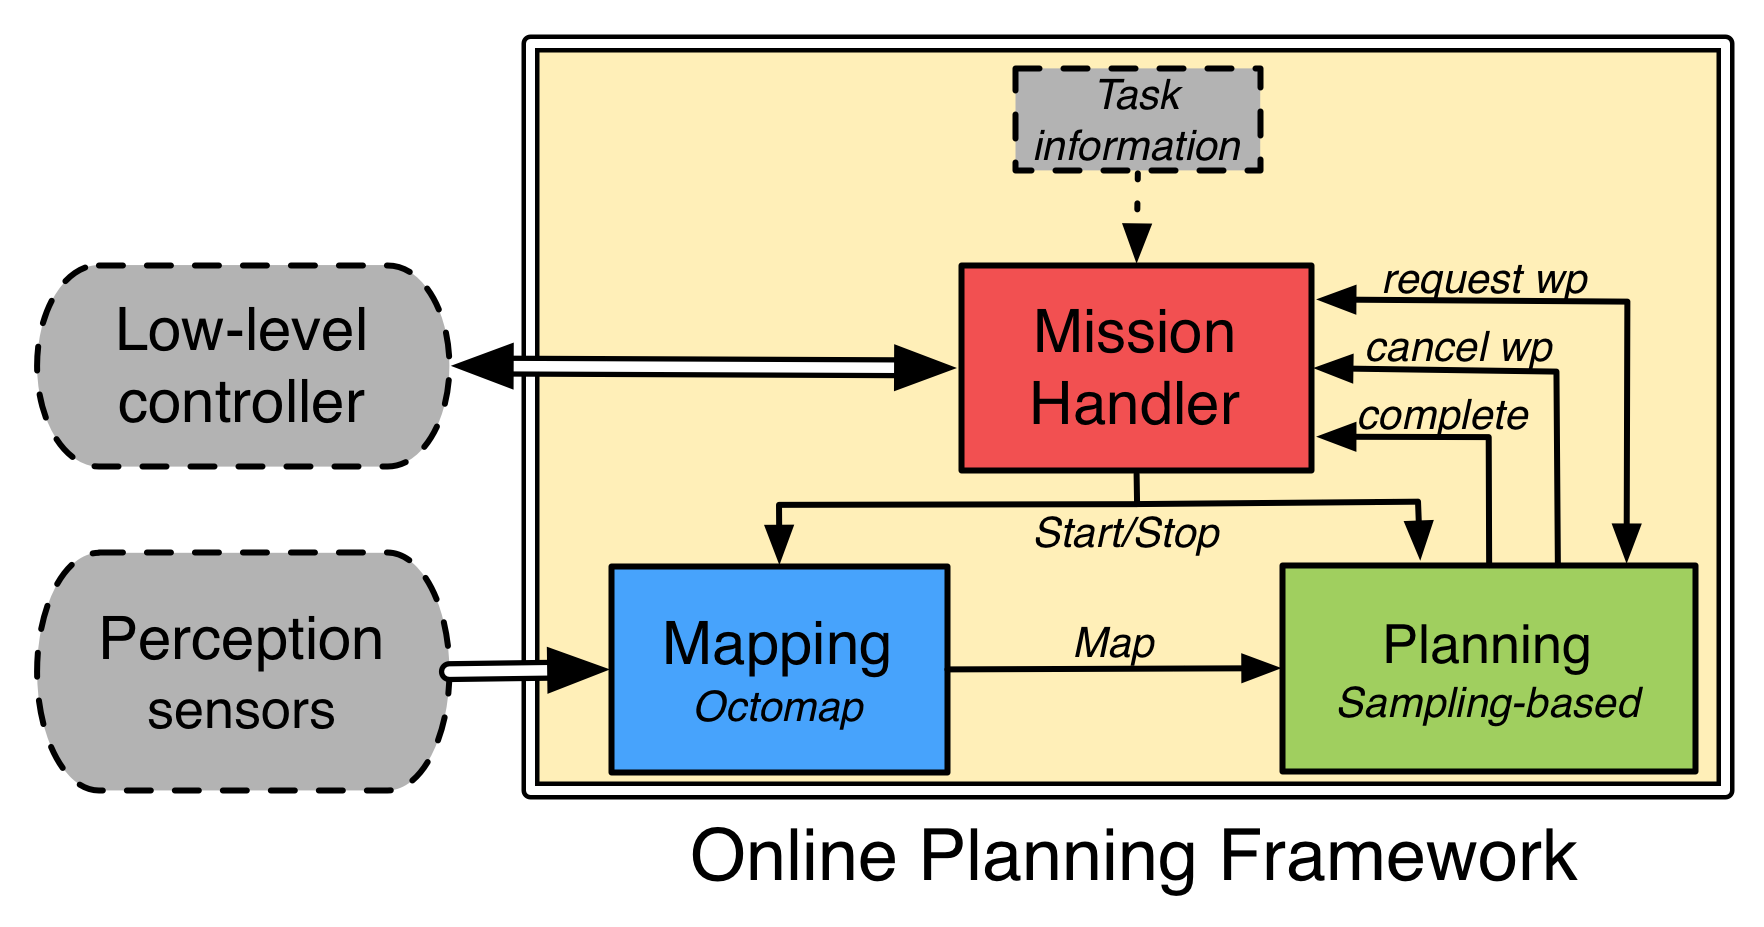
\includegraphics[width=.8\linewidth]{PlanningFramework} \quad
\caption[Framework for online AUV motion planning.]
{Framework for online AUV motion planning.}
\label{fig:ModulesPlannFramework}
\end{figure}

\section{Mission Handler}

The first functional module that constitutes the path/motion planning framework
is the \textit{mission handler}. This module is in charge of controlling and
coordinating the other modules \mbox{(\textit{mapping} and \textit{planning})}.
It also verifies whether the \ac{AUV} is prepared to start solving and
conducting a task. To do so, this module communicates with other functional
modules in the vehicle to verify both that navigation data is correctly being
generated, and that the vehicle low-level controllers are not conducting any
safety maneuvers. After completing this initial checking stage, the
\textit{mission handler} starts requesting waypoints from the \textit{planning}
module, which, after being received, are adapted and sent to the vehicle
low-level controllers. This module is also responsible for cancelling any
ongoing waypoint if it is notified by the \textit{planning} module. This latter
situation will be explained in the following sections.

\section{Module for Incremental and Online Mapping}
\label{sec:MappingModule}

The \textit{mapping} module incrementally builds a representation of the
environment. To do so, it uses data that can be obtained from different kinds of
perception sensors such as multibeam sonars, mechanically scanned profiling
sonars, echosounders, etc. These sensors provide range information about nearby
obstacles that, combined with the vehicle's position and orientation, allows
establishing the free and occupied space with respect to an inertial coordinate
frame. In order to represent this data, this module uses an octree-based
framework called Octomap~\cite{Hornung2013}. This representation has three main
characteristics that efficiently model such volumetric information.

The first characteristic is the probabilistic state representation. This allows
not only to modify the map when updated environment information is available,
but also protects it from noisy measurements. This latter feature is possible
because the state of a particular position over the map considers previous
information, and calculates its new value according to probabilistic functions.
The second characteristic is the capacity of representing unexplored areas,
which can be relevant for guiding the planner over the exploration of unknown
environments. The last characteristic allows an Octomap to be enlarged or
extended as demanded in a computationally efficient way.

Figure~\ref{fig:SantFeliuBlocksOctomap} shows a breakwater structure, which is
located in the harbor of Sant Feliu de Gu\'ixols (Spain), and its representation
with an Octomap that has been built using real-world multibeam sonar data
obtained by a surface vessel. This is one of the test environments used during
the development of this work for both simulated and real-world trials. Results
presented in Chapters~\ref{ch:motion_constratins}~and~\ref{ch:planning_3D}, for
instance, used a virtual scenario and the corresponding Octomap that are based
on this breakwater structure (see Fig.~\ref{fig:CollisionCheck}).

\begin{figure}[htbp]
\myfloatalign
    \subfloat[Breakwater structure]
    {\label{fig:SantFeliuPort}
     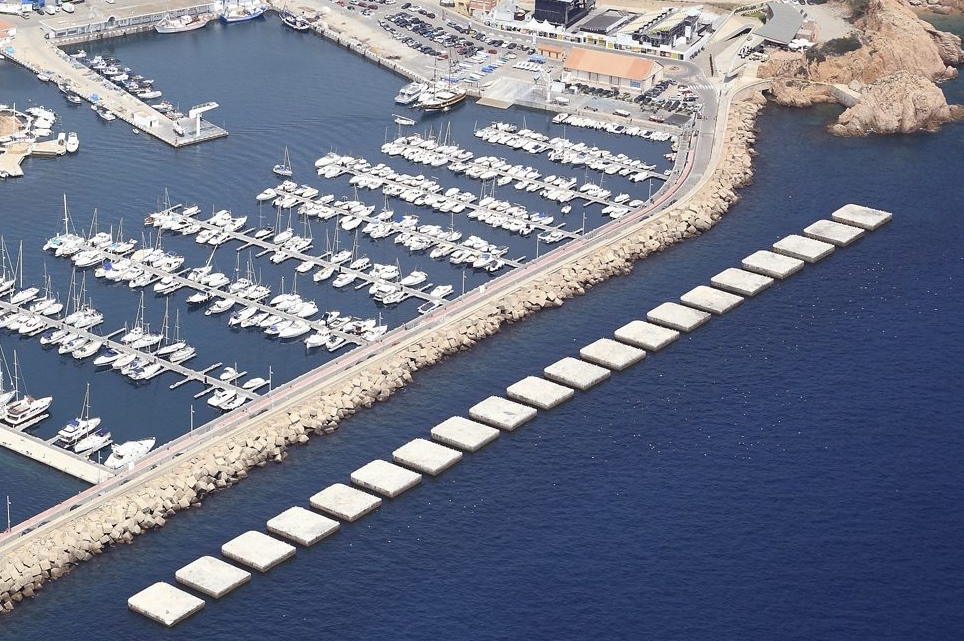
\includegraphics[width=.45\linewidth]{SantFeliuPort}} \quad
    \subfloat[Representation with an Octomap]
    {\label{fig:ConcreteBlocksOctomap}
    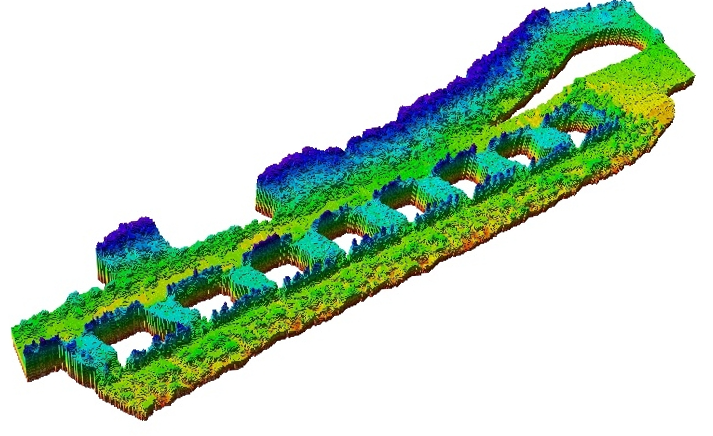
\includegraphics[width=.45\linewidth]{ConcreteBlocksOctomap}}
\caption[Harbor of Sant Feliu de Gu\'ixols (Spain). Aerial view of the
breakwater structure, and a representation of the area with an Octomap.]
{Harbor of Sant Feliu de Gu\'ixols (Spain).
\protect \subref{fig:SantFeliuPort} Aerial view of the breakwater structure.
\protect \subref{fig:ConcreteBlocksOctomap} Octomap representation that has been
created with real-world data acquired with a multibeam sonar.}
\label{fig:SantFeliuBlocksOctomap}
\end{figure}

In order to determine if the vehicle is or would be under collision in a certain
position, the Octomap has to be verified in an equivalent volume that contains
the vehicle. To do so, all voxels within such a volume have to be considered as
non-occupied. This validation can be simplified by representing the \ac{AUV}
volume with one solid such as a cylinder or a hexahedron (see
Fig.~\ref{fig:CollisionCheck}). This collision checking routine between an
Octomap and a solid can be efficiently performed by the \ac{FCL}~\cite{fcl}.

\begin{figure}[htbp]
\myfloatalign
    \subfloat[]
    {\label{fig:CollisionCheckCylinder}
     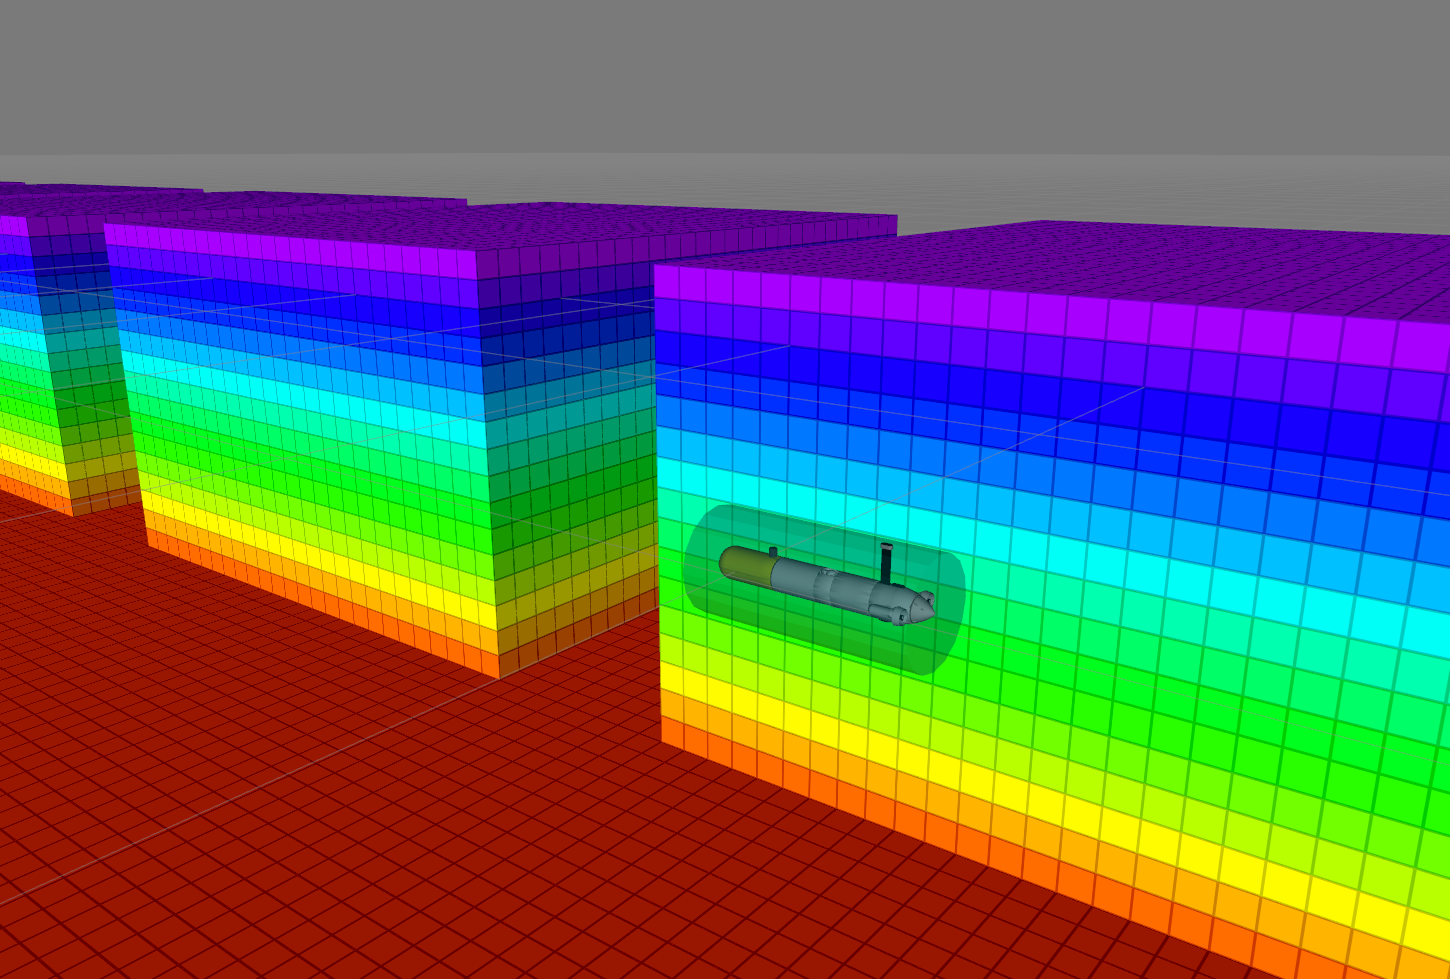
\includegraphics[width=.45\linewidth]{CollisionCheckCylinder}} \quad
    \subfloat[]
    {\label{fig:CollisionCheckCube}
    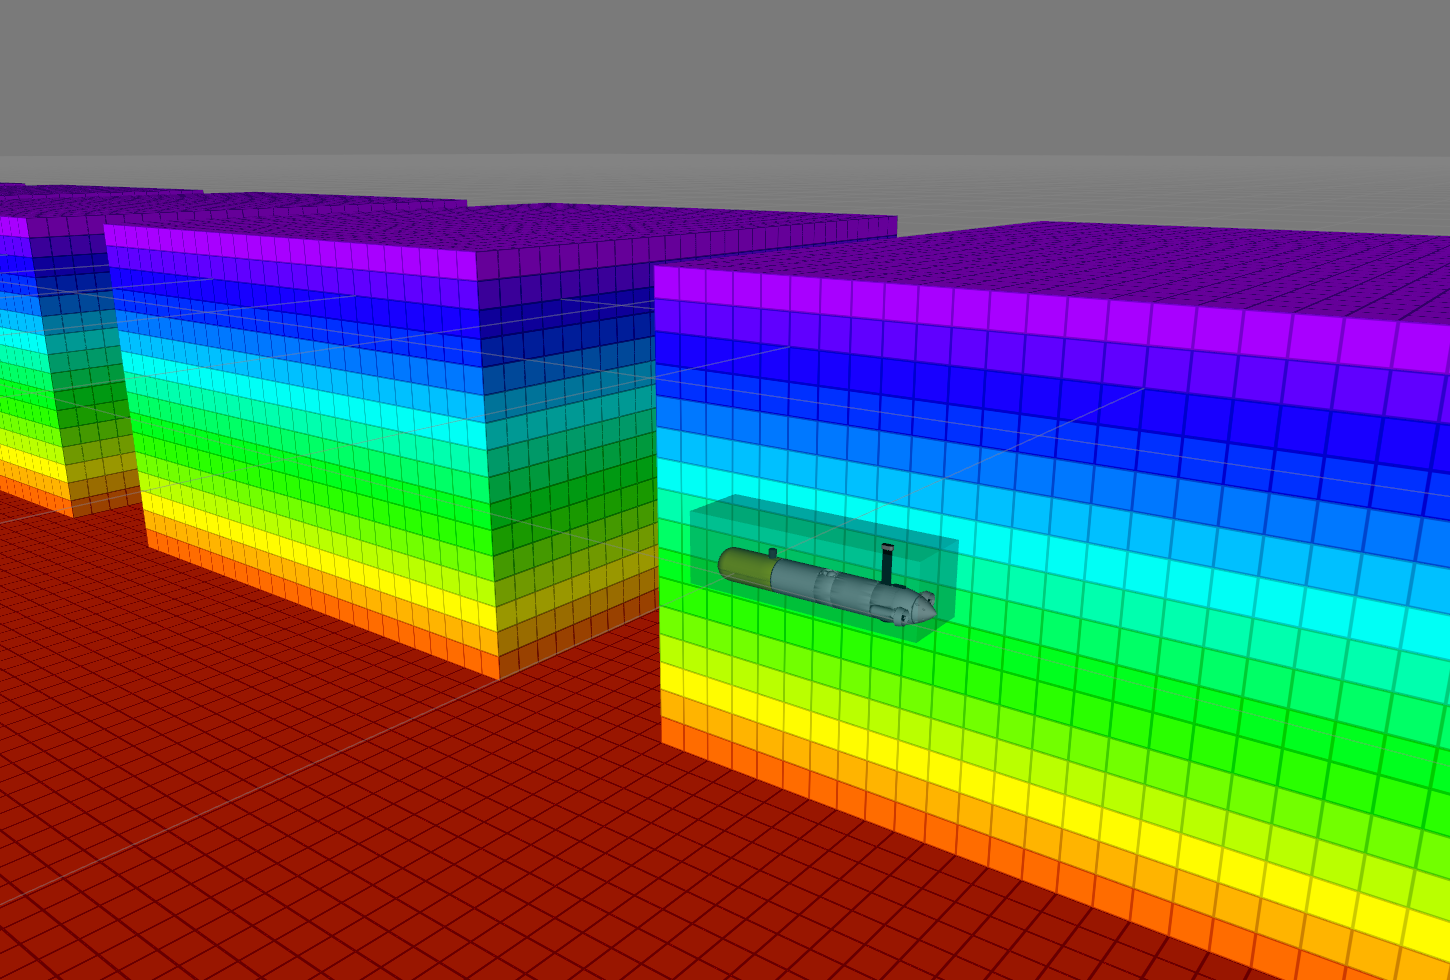
\includegraphics[width=.45\linewidth]{CollisionCheckCube}}
\caption[Collision checking using Octomaps.]
{Collision checking using Octomaps is done by evaluating the Octomap voxels that
contain the equivalent volume of the AUV. In order to simplify this validation
routine, the AUV volume can be represented by a solid such as a \protect
\subref{fig:CollisionCheckCylinder} cylinder or a \protect
\subref{fig:CollisionCheckCube} hexahedron.}
\label{fig:CollisionCheck}
\end{figure}

\section{Module for (Re)Planning Paths Online}

The third functional module of the proposed framework is the \textit{planning}
module, which is in charge of calculating a collision-free and feasible path for
the \ac{AUV}. For doing so, this module receives a query that is specified with
a start configuration ($q_{start}$) and a goal configuration ($q_{goal}$), and
other parameters, such as the available computing time and the minimum valid
distance to the goal. Furthermore, given that the vehicle navigates in an
unexplored (or unknown) environment, this module must continuously verify and
repair (if necessary) the path from the current vehicle configuration to
$q_{goal}$. In order to calculate a path under such constraints, this module
contains a modified implementation of the \ac{RRT*} algorithm.

This \ac{RRT*} variant not only permits to progressively improve the solution,
but it has also been extended to safely navigate while efficiently replanning
the path as the environment is incrementally explored. Our extensions include an
optimization function that combines collision risk and path length; a strategy
to avoid unnecessary and expensive state checking routines; and the reuse of the
last best known solution as a starting point for an anytime planning approach.
These new characteristics are presented and explained in detail in the following
sections.

\subsection{Planning Safe Paths using Risk Functions}
\label{sec:RiskFunctions}

Conducting underwater missions with \acp{AUV} is a challenging task, especially
when the vehicle is kinematically constrained, as it was explained in
Chapters~\ref{ch:motion_constratins}~and~\ref{ch:planning_3D}. However,
including motion constraints to the path planner may not suffice to
minimize the risk of colliding with nearby obstacles. This is especially true
when the vehicle is exposed to external perturbations, which do not permit the
\ac{AUV} to accurately follow the calculated path.
Figure~\ref{fig:GeomRRTstarDubPathLeng_Rviz}, for instance, shows a feasible
path, \ie one that considers the vehicle motion constraints. However, as the
solutions are only asymptotically optimized with respect to their length, they
lead the vehicle close to nearby obstacles, especially in turning maneuvers.

\begin{figure}[htbp]
	\centering
	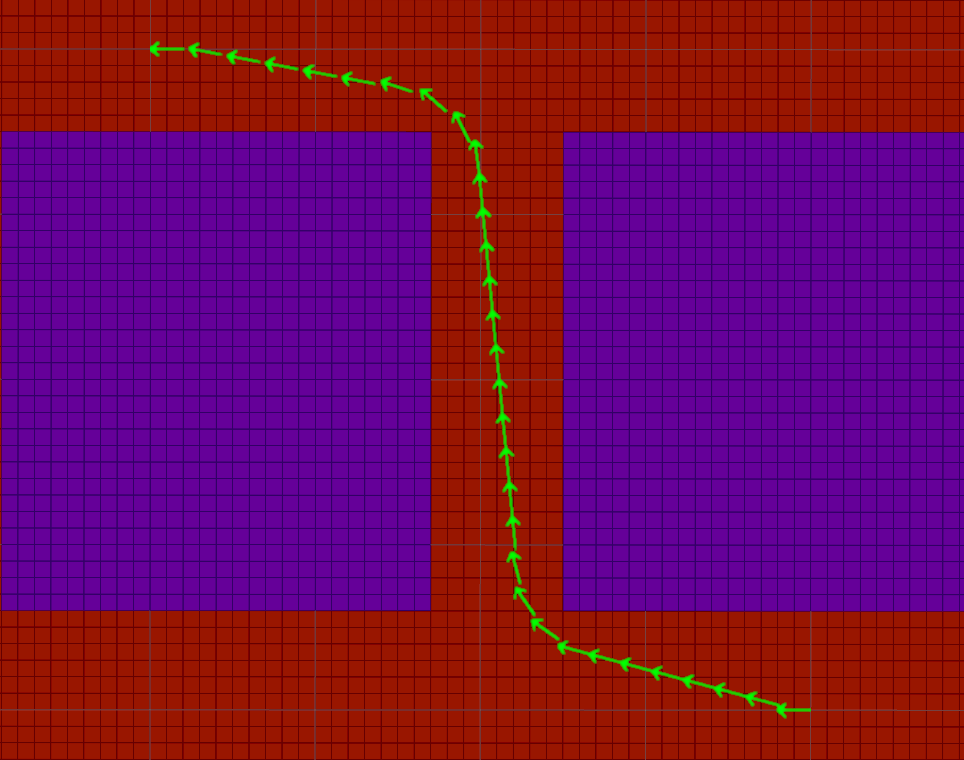
\includegraphics[width=.45\linewidth]{GeomRRTstarDubPathLeng_Rviz}
\caption[A start-to-goal query solution using an RRT* algorithm with Dubins
curves.]
{A start-to-goal query solution that was calculated by an \ac{RRT*} algorithm
with Dubins curves as steering function. The solution path requires the vehicle
to move close to nearby obstacles when conducting turning maneuvers.}
\label{fig:GeomRRTstarDubPathLeng_Rviz}
\end{figure}

Bearing this in mind, the objective would be now to extend the planner to not
only plan feasible paths, but also to attempt to minimize the risk of colliding
with the surroundings. To accomplish this, one alternative is to provide an
optimization objective to the planner that combines the length and the safety
of the path. The following sections present different approaches to achieve
this.

\subsubsection{Path Length + Clearance}

A first and straightforward option is to maintain a minimum safe distance, or
clearance, to the obstacles. For doing so, it is necessary to establish a
weighted metric that combines path length and clearance in order to minimize
detrimental effects in the path quality. This allows us to define the associated
cost of each configuration when planning with an \ac{RRT*} algorithm. However,
this approach has two main drawbacks, its high computational cost and the need to
correctly specify weights to obtain a balanced metric, which is a non-trivial
problem~\cite{Tsianos2007}.

\subsubsection{Risk Zones}

Including clearance calculation is especially expensive for sampling-based
path/motion planning methods, since it has to be performed for each sampled
configuration and its intermediate steps when connecting to the others (\eg
\ac{RRT*} algorithm expansion). One alternative is to heuristically establish
risk zones around the vehicle, as shown in Fig.~\ref{fig:RiskZones}.

\begin{figure}[htbp]
	\centering
	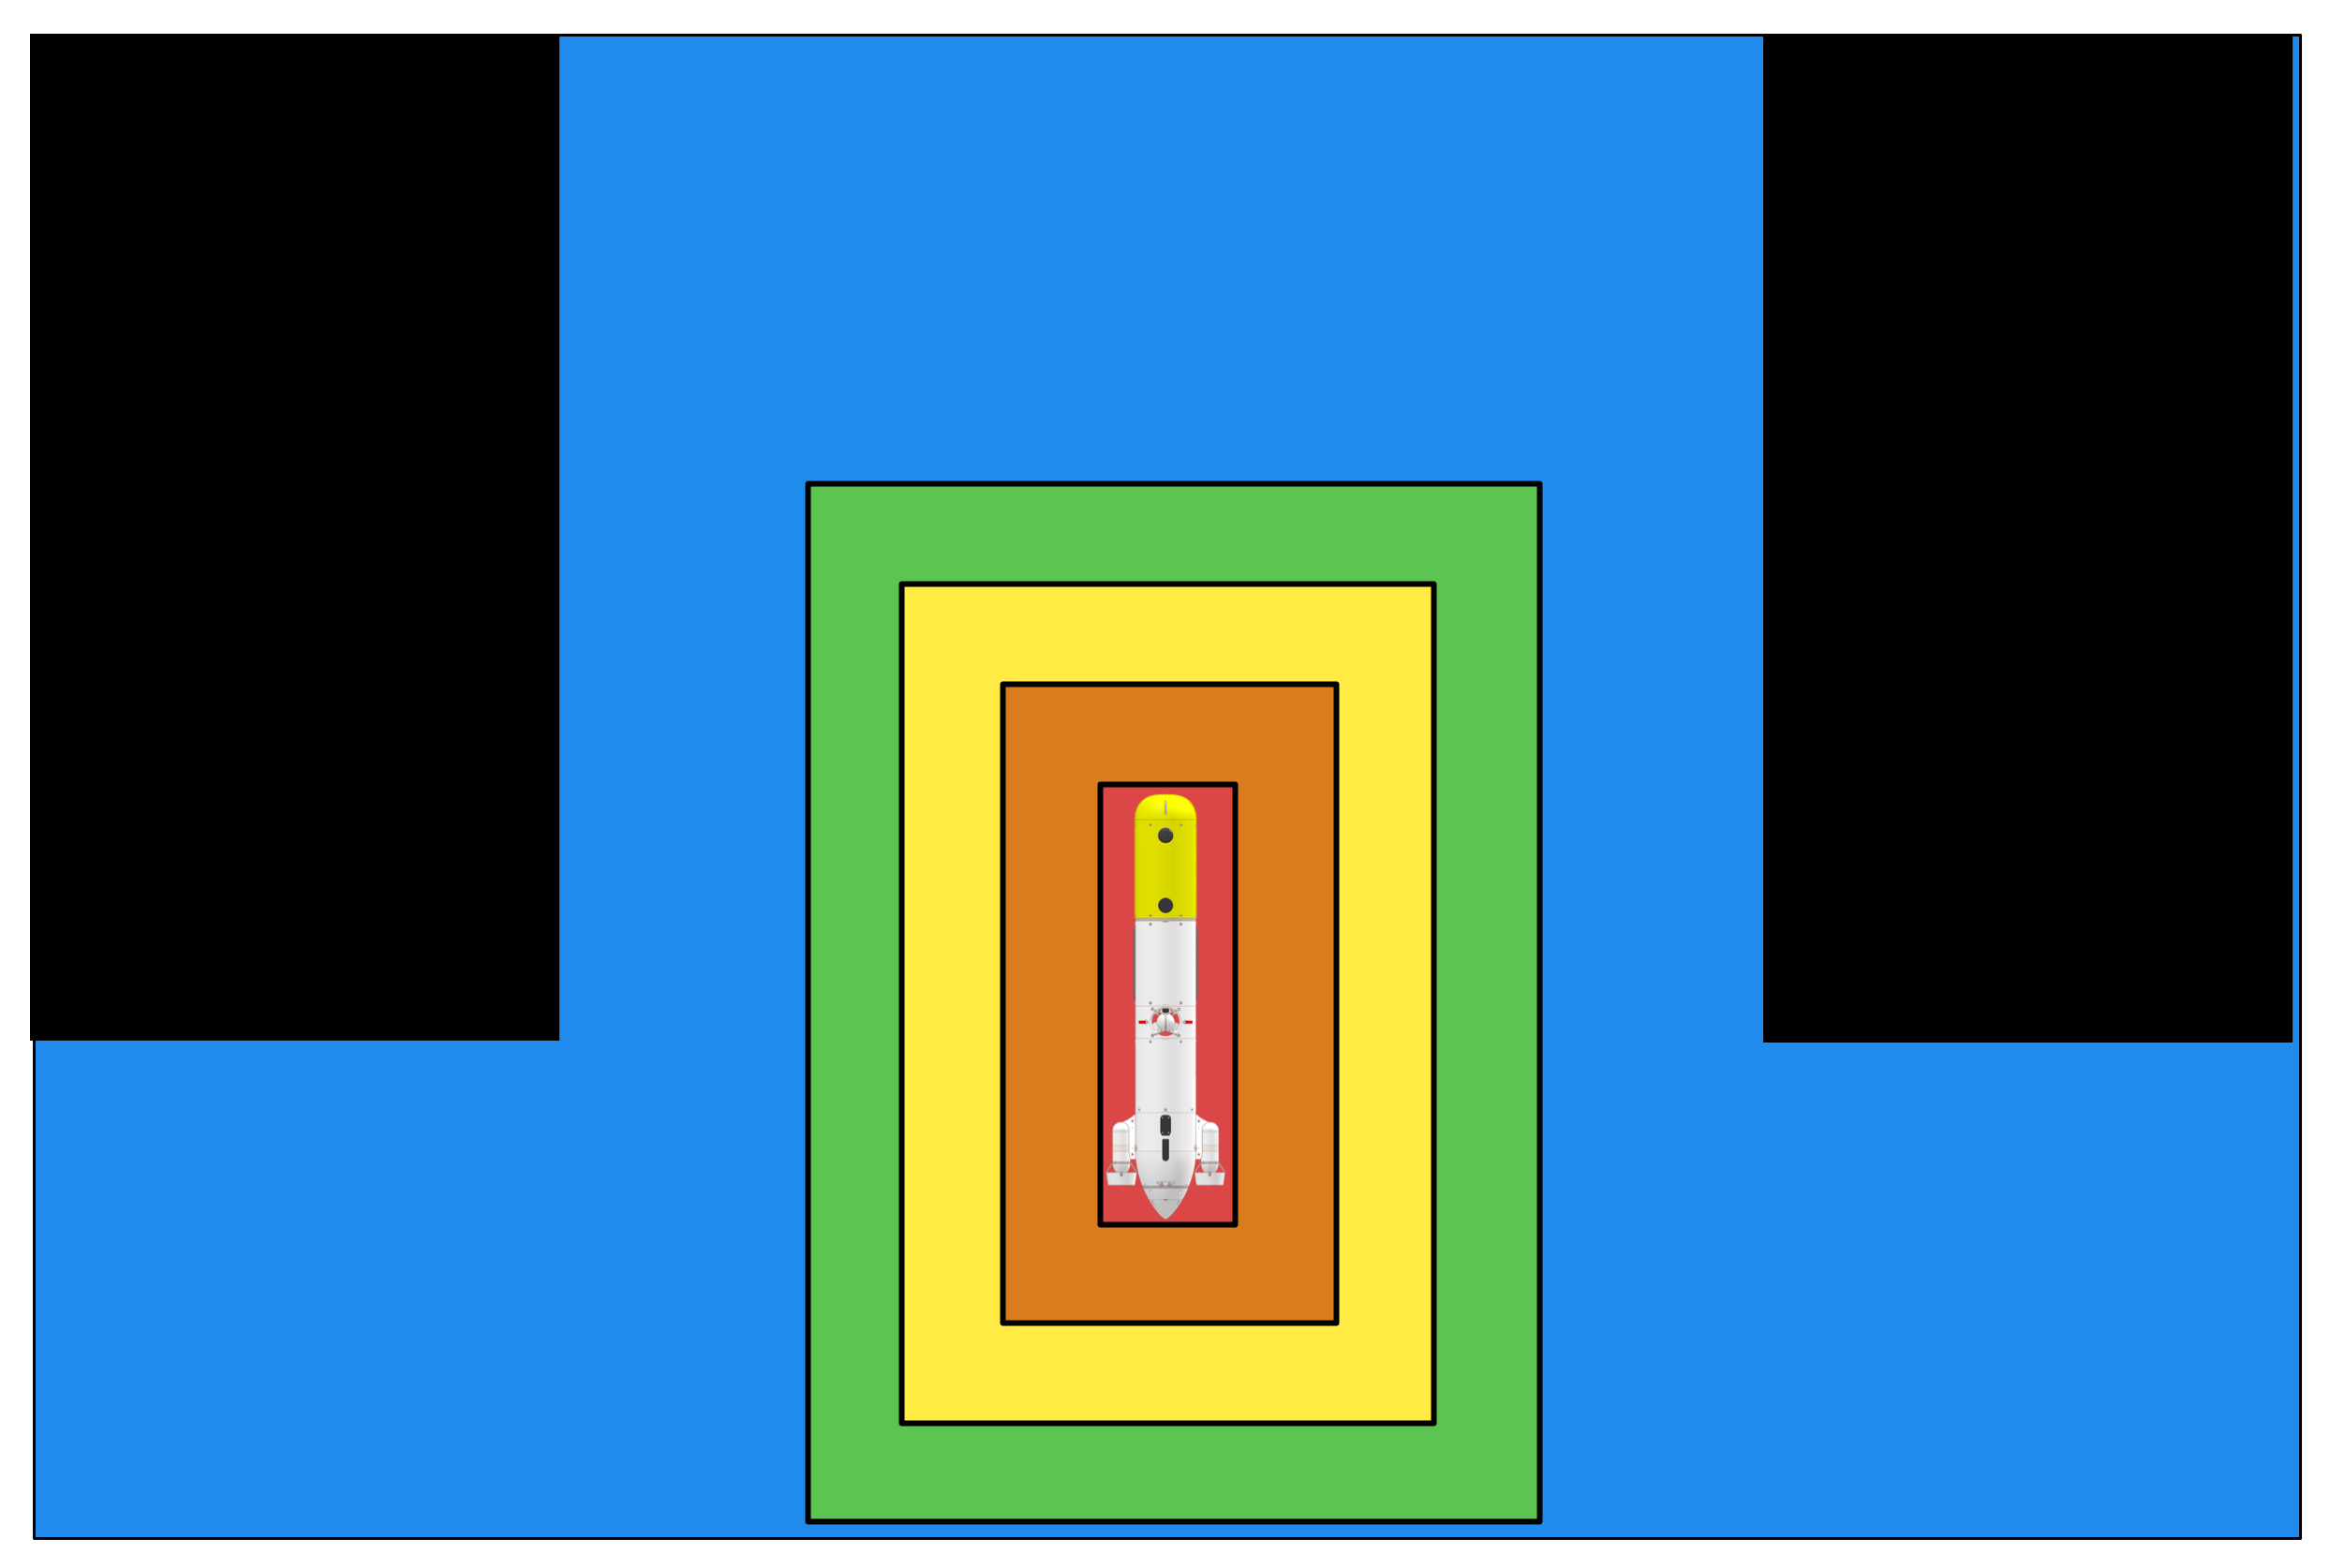
\includegraphics[width=.6\linewidth]{RiskZones}
\caption[Sparus~II AUV navigating between two obstacles and a visual
representation of the risk zones around the vehicle.]
{Sparus~II \ac{AUV} navigating between two obstacles (black). An example of the
risk zones around the vehicle, and how the risk decreases as moves away from the
vehicle can be observed (red means high risk, while blue low risk).}
\label{fig:RiskZones}
\end{figure}

The red and blue zones represent the collision and the non-risk zones,
respectively, while the others (orange, yellow and green) have associated
decreasing risk values as collisions move away from the vehicle position.
Therefore, the risk associated with a given configuration $q$, can be
represented by Eq.~\eqref{eq:risk}, where $n$ is the number of zones,
$zone_{i-1}$ is closer than $zone_{i}$ to the collision zone,
$risk_{i-1}>risk_{i}>\ldots>risk_{n}>1$.

\begin{align} 
	\label{eq:risk}
	Risk(q)=
	\begin{cases}
		risk_1, & if\ Collision(zone_1)\\
		risk_2, & if\ Collision(zone_2)\\
		\ldots, & \ldots\\
		risk_n, & if\ Collision(zone_n)\\
		1, & if\ not\ Collision(any\ zone)\\
	\end{cases}
	\notag\\
	q=[x,y,z,\psi]^T
\end{align}

In order to combine this function with the path length, the total accumulated
cost associated with each configuration is calculated as the integral of risk
with respect to distance, as presented in Eq.~\eqref{eq:cost}. Such a cost
function not only combines the risk and the length associated with a path, but
it also establishes the optimization criterion required in order to plan feasible
and safe paths. A visual comparison between paths calculated using only the path
length and the those with risk zones can be observed in
Fig.~\ref{fig:GeomRRTstarSafe}.

\begin{equation}
	\label{eq:cost}
	Cost(q)=\int_{0}^{q} Risk(q)\, \mathrm{d}q	
\end{equation}

% Finally, it is important to highlight that checking for collision from the inner
% to the outer zone, for a limited number of zones, is computationally more
% efficient than calculating position clearance. This is especially true when the
% environment is not described with a simplified representation (\eg convex
% obstacles), where distance to obstacles can be rapidly calculated, but
% instead a more detailed representation is used (\eg Octomaps).

\begin{figure}[htbp]
\myfloatalign
    \subfloat[]
    {\label{fig:GeomRRTstarDubPathLeng}
     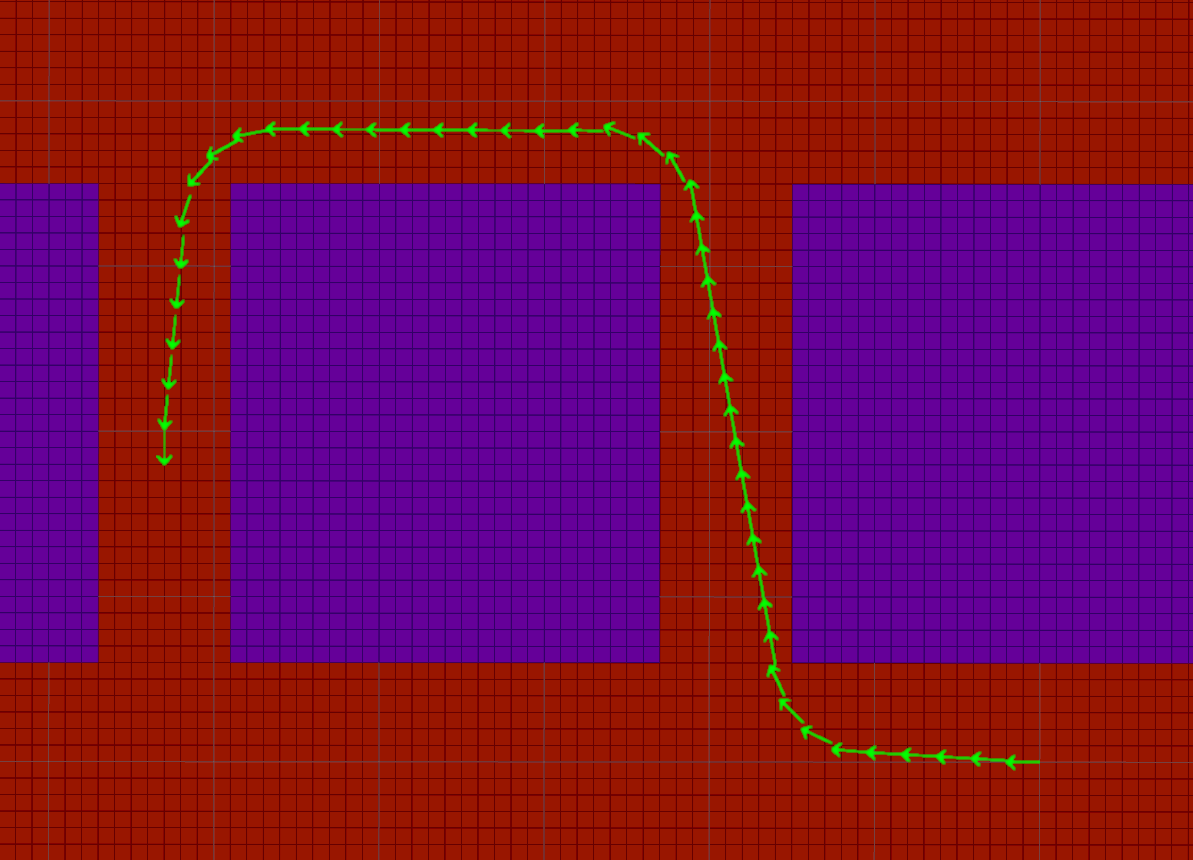
\includegraphics[width=.45\linewidth]{GeomRRTstarDubPathLeng}} \quad
    \subfloat[]
    {\label{fig:GeomRRTstarDubPathLengRiskZones}
    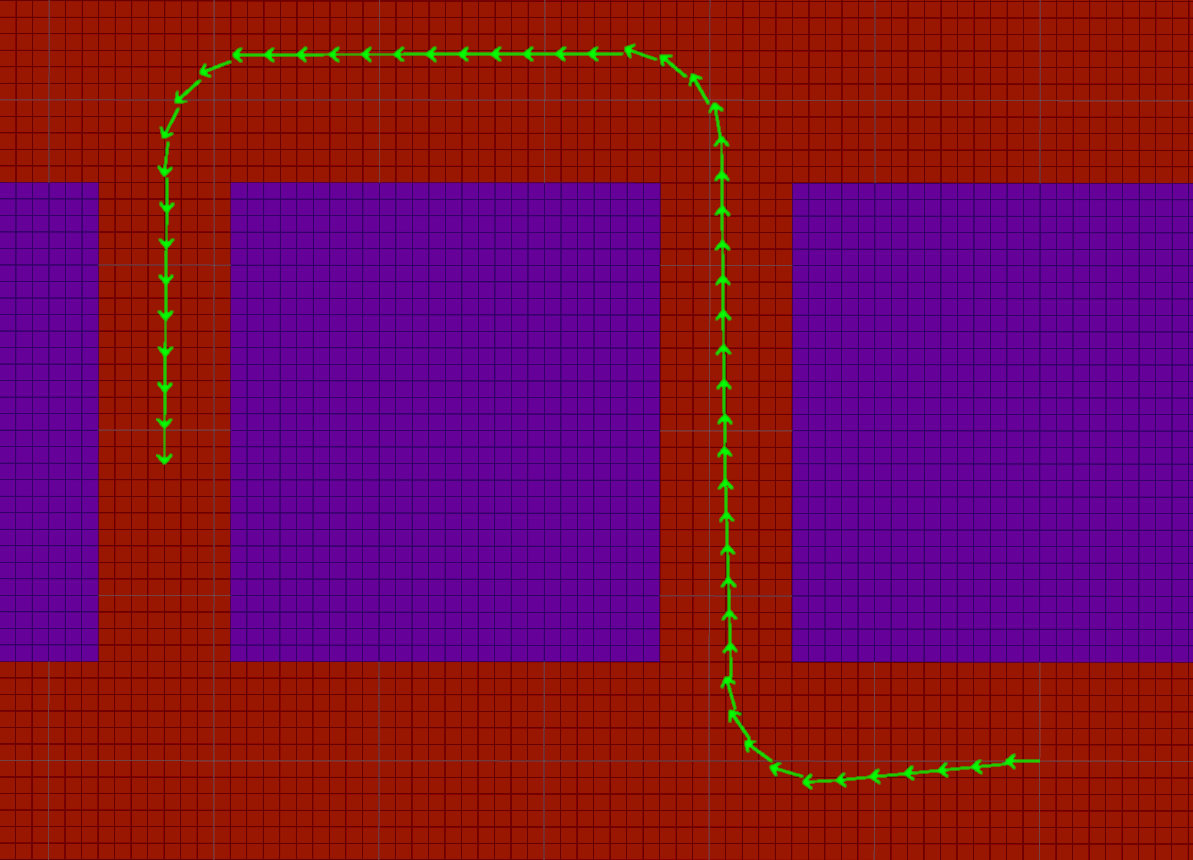
\includegraphics[width=.45\linewidth]{GeomRRTstarDubPathLengRiskZones}}
\caption[Start-to-goal queries' solutions obtained by RRT* with Dubins curves.
Optimization criteria comparison between path length and risk zones.]
{\protect\subref{fig:GeomRRTstarDubPathLeng} RRT* expansion for a start-to-goal query using Dubins curves with path length as cost criterion.
\protect\subref{fig:GeomRRTstarDubPathLengRiskZones} RRT* expansion with
risk zones cost criterion. It is worth noting that the resulting path is far
from corners in turning maneuvers and attempts to stay in the middle of the
corridor when navigating between two obstacles.}
\label{fig:GeomRRTstarSafe}
\end{figure}

\subsubsection{Risk Vectors} 

The previous approach attempts to penalize those configurations close to nearby
obstacles by specifying a risk value, which depends on the affected zone.
However, another alternative is to limit such evaluation to the directions
defined by the possible maneuvers of the vehicle at the considered time. To do
this, let us define three vectors in the straight and lateral motion directions.
Now, instead of checking for complete zones, only points along those vectors
will be checked for collision, assigning risk values with the same principle as
done with risk zones, \ie moving away from the vehicle decreases the risk (see
Fig.~\ref{fig:RiskDirectionVectors}). This approach is here called \textit{risk
vectors}. It is computationally a less expensive alternative, given that
checking collision for single points is more efficient than doing the check for
zones (multiple points), especially when using of Octomaps to represent the
environment.

\begin{figure}[htbp]
	\centering
	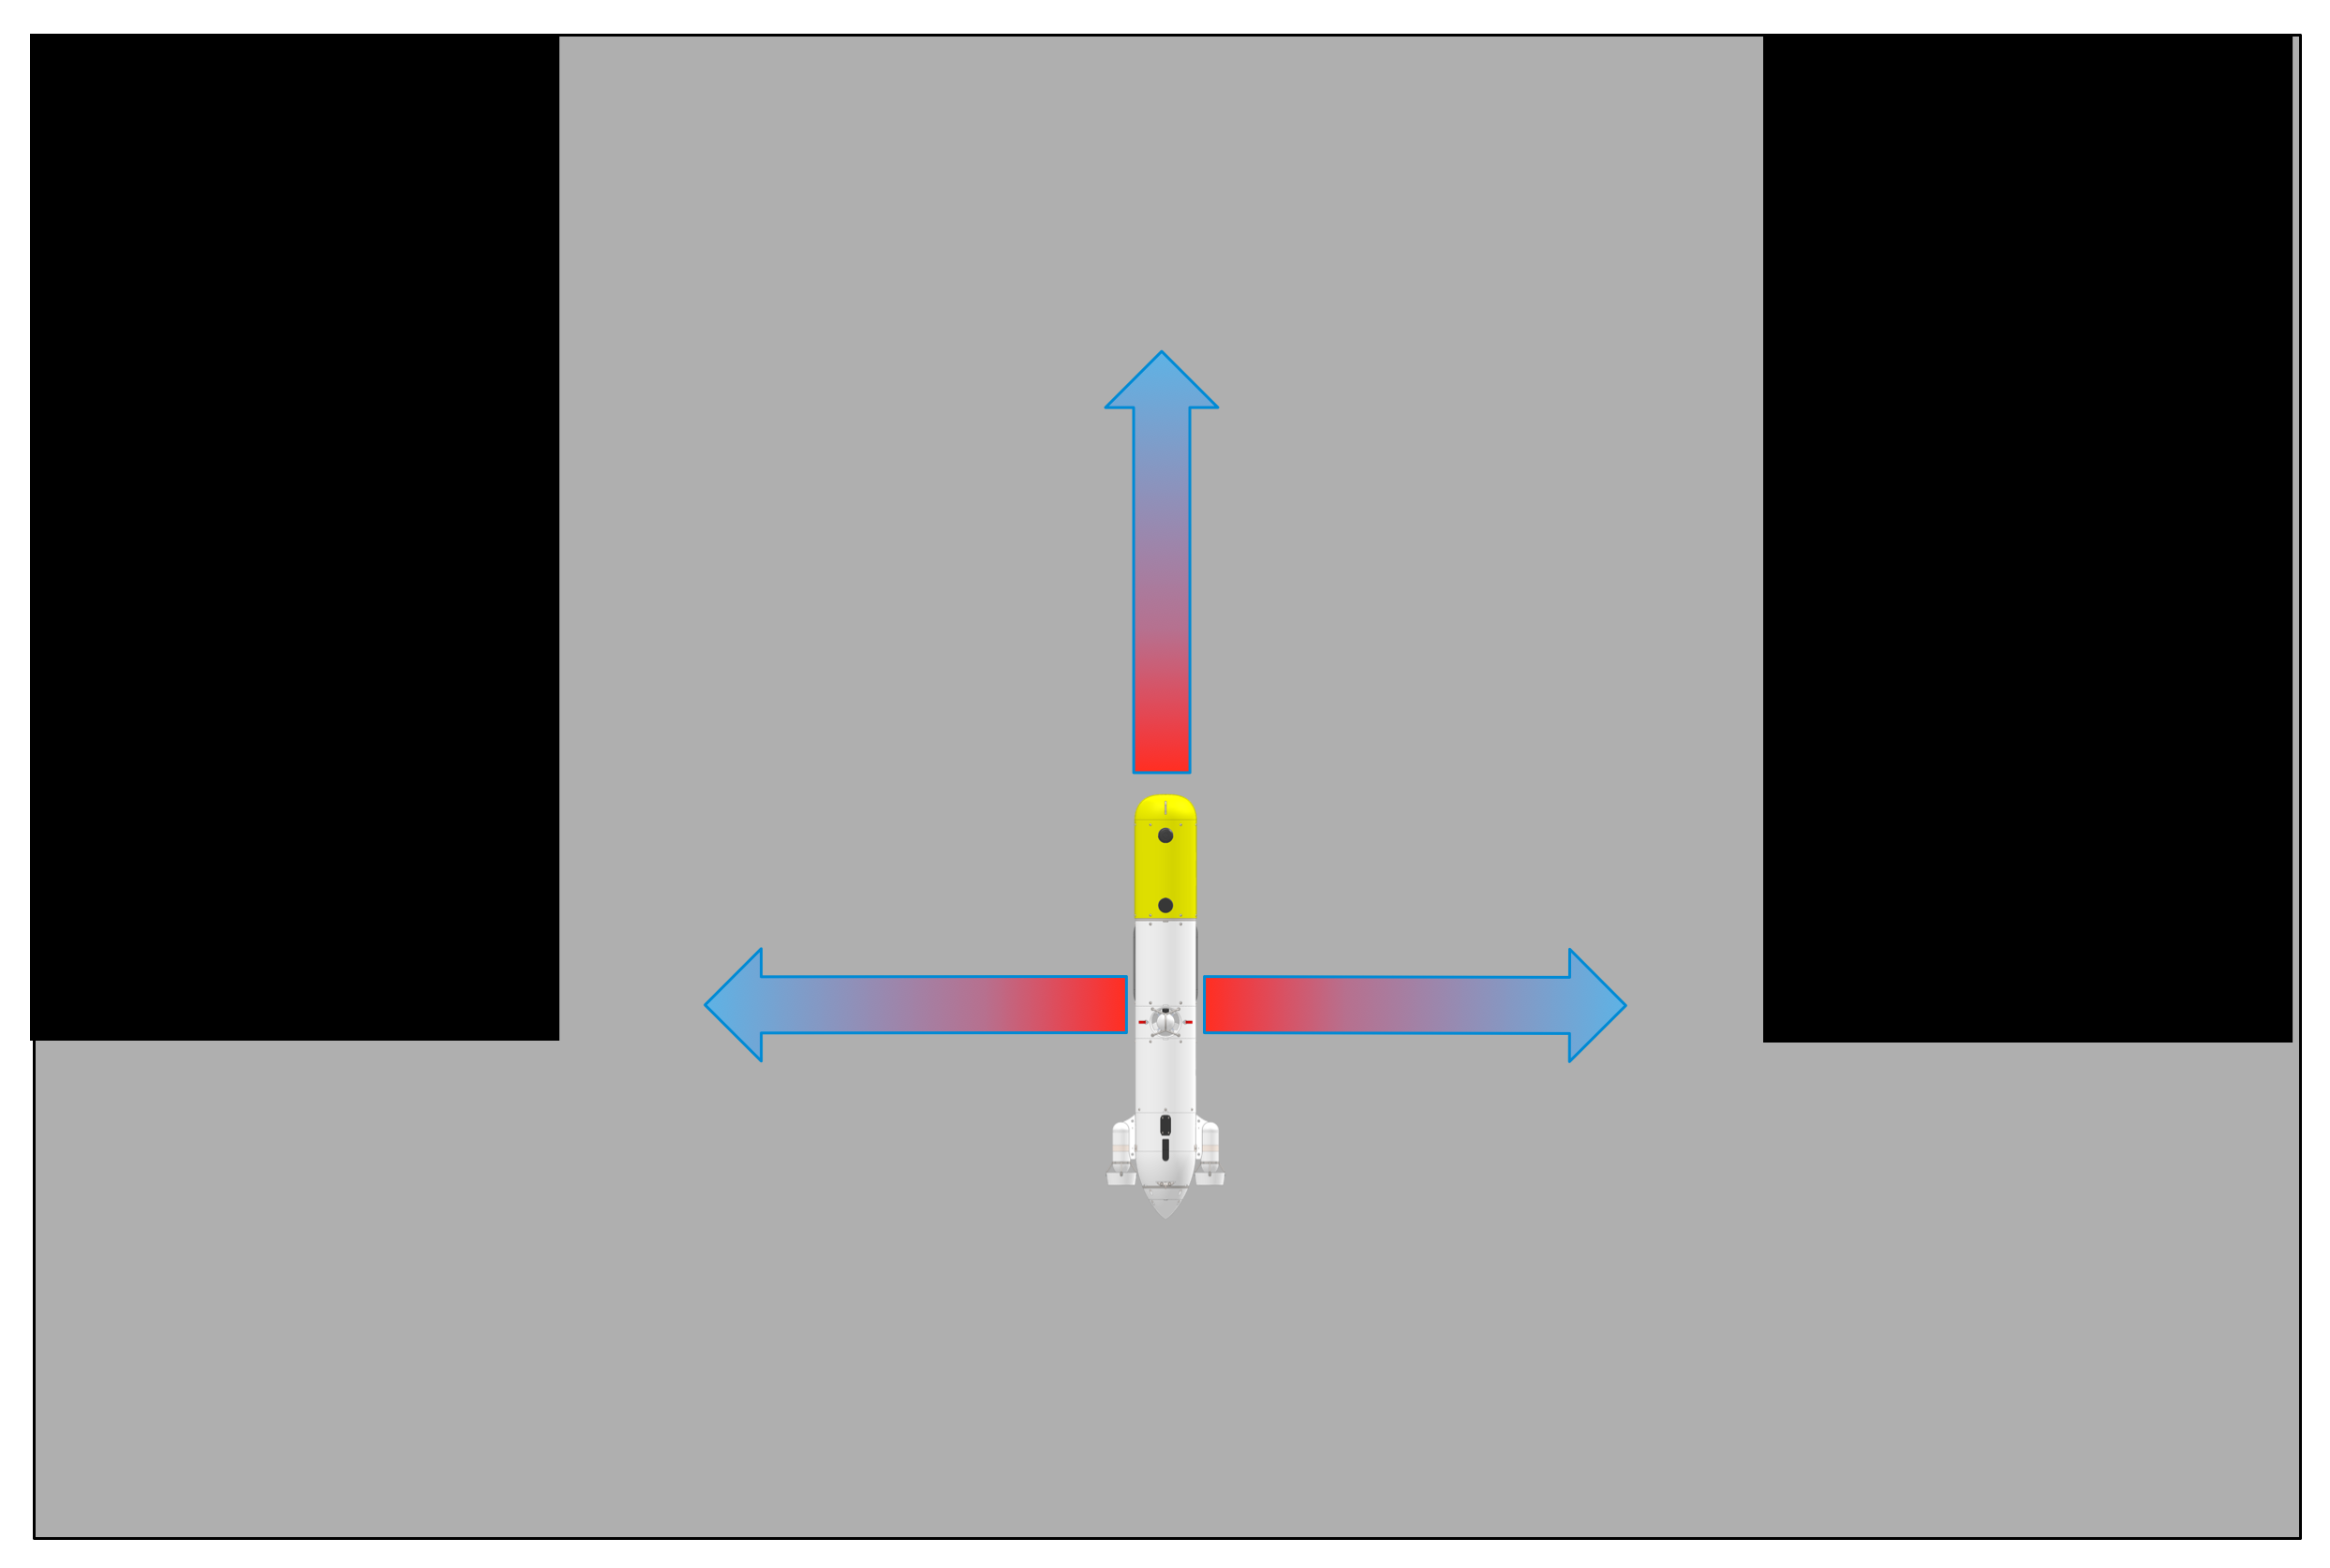
\includegraphics[width=.6\linewidth]{RiskDirectionVectors} 
\caption[Sparus~II AUV navigating between two obstacles and a visual
representation of the risk vectors zones around the vehicle.]
{Sparus~II \ac{AUV} navigating between two obstacles (black). An example of the
risk vectors, and how the risk decreases as moves away from the vehicle can be
observed (red means high risk, while blue low risk).}
\label{fig:RiskDirectionVectors}
\end{figure}

Both the risk zones and the risk vectors have also been extended for \ac{3D}
motions. In the case of the risk zones, the areas around the vehicle become
volumetric shapes of increasing size (\eg rectangular prisms, or cylinders),
whereas with the risk vectors it is enough to add the corresponding vectors for
the vertical motion (see Fig.~\ref{fig:3DRiskZonesVectors}). These alternatives
to quantify the risk associated with a path have been evaluated and compared
with each other. The results of this analysis will be discussed in
Sec.~\ref{sec:PlanningOnlineResults}.

\begin{figure}[htbp]
\centering
    \subfloat[3D risk zones.]
    {\label{fig:3DRiskZones}
     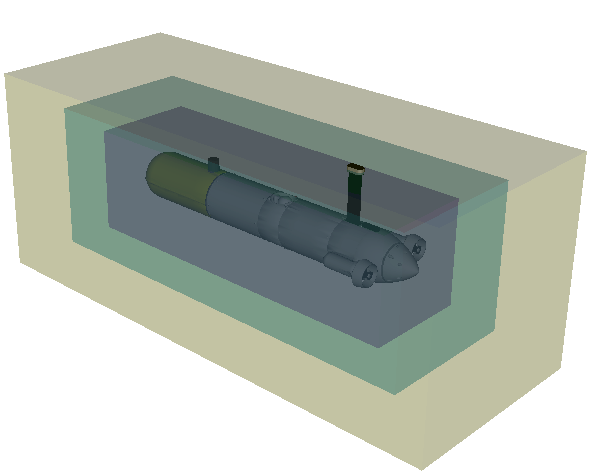
\includegraphics[width=.45\linewidth]{3DRiskZones}} \quad
    \subfloat[3D risk vectors.]
    {\label{fig:3DRiskVectors}
    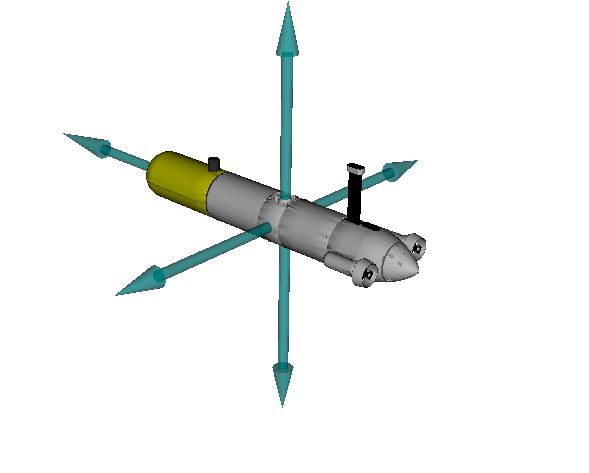
\includegraphics[width=.45\linewidth]{3DRiskVectors}}
\caption[Extension of risk zones and risk vectors for 3D motions.]
{Extension of risk zones and risk vectors for 3D motions.}
\label{fig:3DRiskZonesVectors}
\end{figure}

\subsection{Opportunistic State Checking}
\label{sec:OportStateCheck}

Previous sections presented the estimation of the risk associated with a path,
which is the first main characteristic of the proposed framework and its
\textit{planning} module. This section, on the other hand, introduces the second
characteristic that seeks to optimize the computation time in missions where the
environment is incrementally explored.

When conducting an autonomous mission without initial information of the
surroundings, the \ac{AUV} is required to incrementally map and continuously
(re)plan collision-free paths according to its partial knowledge of the
environment. Because of this, and assuming the \textit{planning} module uses a
sampling-based method such as the \ac{RRT*} algorithm, an important number of
configurations (sampled or obtained after expanding the tree) are located in
unexplored regions of the environment. In these situations, it is not only
impossible but also unnecessary to attempt to determine if a configuration is at
risk of collision. In order to compensate this, one alternative is to assume as
safe (collision-free and minimum risk) any configuration that is out of the
explored area. This can be efficiently determined when using Octomaps (as
explained in Section~\ref{sec:MappingModule}). This strategy, proposed in this
thesis, is called \textit{opportunistic state checking}, and is inspired by the
\textit{lazy collision checking} (which was explained in
Sec.~\ref{sec:lazy_collision_check}).

Figure~\ref{fig:OpportStateCheck} depicts a simulation where the explored and
free regions of the map are presented in light blue, the occupied ones are
presented in purple, and the rest correspond to unexplored areas. With this
visualization, it is possible to observe the importance of avoiding checking for
collision of those configurations that are located in undiscovered regions.
Section~\ref{sec:PlanningOnlineResults} will show different tests that
demonstrate the advantages of using this strategy.

\begin{figure}[htbp]
\myfloatalign
    \subfloat[]
    {\label{fig:OpportStateCheck1}
     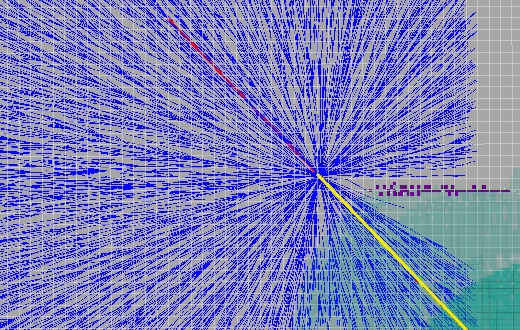
\includegraphics[width=.45\linewidth]{OpportStateCheck1}} \quad
    \subfloat[]
    {\label{fig:OpportStateCheck2}
    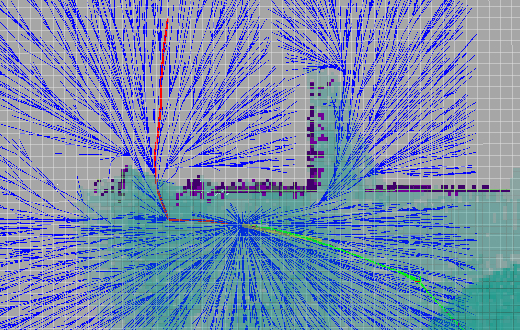
\includegraphics[width=.45\linewidth]{OpportStateCheck2}}
\caption[Opportunistic state checking. An important number of configurations
are located in unexplored regions.]
{Sparus II AUV conducting an autonomous mission in the simulated
breakwater structure scenario without an initial map.
\protect\subref{fig:OpportStateCheck1} The explored region, presented in light
blue, expands as the vehicle moves towards the goal. It is important to notice
that a significant part of the tree (dark blue) is located in unexplored areas
of the workspace. \protect\subref{fig:OpportStateCheck2} Those branches are
initially assumed as safe (collision-free) until the corresponding region is
explored, thus avoiding unnecessary collision-checking routines~computation.}
\label{fig:OpportStateCheck}
\end{figure}

In this incremental mapping and planning approach, the tree expansion is
periodically interleaved with updating the map, and such parts initially assumed
as safe must be verified and discarded if found under collision as the vehicle
explores the environment (a situation that can also be observed in
Fig.~\ref{fig:OpportStateCheck}). The next section describes and analyses two
alternative mechanisms to check and reshape the tree.

\subsection{Reuse of the Last Best Known Solution}
\label{sec:ReuseLastBestKnownSol}

This section presents the \textit{reuse of the last best known solution}, which
is the third main characteristic of the proposed framework and its
\textit{planning} module. Such a strategy allows an incremental and tree-based
path planner, such as the \ac{RRT*} algorithm, to replan or reshape the solution
path according to the new environment information perceived during the mission.
However, in order to fully understand the benefits associated with this
strategy, this section firstly explains another alternative that was initially
used, but later discarded due to its high computational cost.

\subsubsection{Pruning the Tree for Anytime Computation}

One alternative for dealing with partially known environments is to grow a
single tree of collision-free configurations (as any \ac{RRT} variant does),
while periodically pruning the tree. This process allows discarding those
branches that result under collision after updating the map, thus obtaining a
valid solution at \textit{anytime} that is requested. This strategy has been
used with approaches based on the \ac{RRT}~\cite{Bekris2007} and the
\ac{RRT*}~\cite{Karaman2011a}. At a first stage of this thesis, the
\textit{planning} module used a modified \ac{RRT*} algorithm that was based on
this pruning approach.

Like other \ac{RRT}-based algorithms, the initially used variant consisted of
two procedures, \texttt{sample} and \texttt{extend} (see Sec.~\ref{sec:RRT}).
However, the former one had two main modifications (see
Algorithm~\ref{alg:SampleAnytimeRRT}). The first one was intended to correct the
tree according to the new elements discovered in the environment. To do so, and
before sampling new configurations, the \texttt{updateTree} procedure traversed
the tree using a \ac{DFS} algorithm to check if any node or edge was under
collision (line~\ref{lin_alg:UpdateTree}). If a new collision was detected, the
corresponding subtree (\ie those branches with nodes or edges under collision)
was discarded. However, if the tree root was one of the nodes under collision,
or if the path from the current vehicle configuration to the root was not
feasible, the \textit{planning module} informed the \textit{mission handler} to
cancel the current path followed by the controller, and then it started again
planning a new path from the current vehicle position. This latter situation
occurred because the tree root always corresponded to the configuration (or
position) that the vehicle was moving towards.

The purpose of the second modification in the \texttt{sample} procedure was to
make the \ac{RRT*} behave as an \textit{anytime} algorithm. To do this, if the
new configuration $q_{new}$ resulted from the tree expansion met the specified
minimum distance to the goal (line~\ref{lin_alg:CondSolRRT}), it was added to a
list of possible solutions (line~\ref{lin_alg:AddSolRRT}). Furthermore, if the
\textit{mission handler} had requested a new waypoint after concluding the tree
expansion, and there was at least one available solution stored in the list
(line~\ref{lin_alg:CondReqRRT}), the planner selected the solution with the
minimum associated cost, sent the \textit{mission handler} the configuration
connected to the root of that solution (line~\ref{lin_alg:SendWpRRT}), and
pruned the tree in such a way that the configuration sent became the new tree
root (line~\ref{lin_alg:PruneRRT}). During this \textit{pruning} process,
subtrees connected to the former root (excepting the one that corresponds to the
new root) were discarded. The \texttt{extend} procedure, on the other hand, remained
as originally proposed in~\cite{Karaman2011}.

\begin{algorithm}[H]
	\DontPrintSemicolon
	\SetKwFunction{updateTree}{updateTree}
	\SetKwFunction{sampleConf}{sampleConf}
	\SetKwFunction{extendRRT}{extendRRT*}
	\SetKwFunction{updateBestSolution}{updateBestSolution}
	\SetKwFunction{dist}{dist}
	\SetKwFunction{getBestSolution}{getBestSolution}
	\SetKwFunction{sendWaypoint}{sendWaypoint}
	\SetKwFunction{pruneTree}{pruneTree}

	\KwIn{\\ 
	$q_{start}:$ Start configuration. \\
	$q_{goal}:$ Goal configuration.\\
	$\mathcal{C}$: \ac{C-Space}.}
	
 	\Begin{
 		\updateTree{}\;\label{lin_alg:UpdateTree} 
 		\While{not $stop\_condition$}{
  			$q_{rand}\leftarrow$\sampleConf{}\label{lin_alg:SampleRRT}\;
  			$result,q_{new}\leftarrow$\extendRRT{$T,q_{rand}$}\;\label{lin_alg:ExtendRRT}
  			\If{$result \neq \text{TRAPPED}$} {
  				\If{\dist{$q_{new}, q_{goal}$} $< \epsilon_{goal}$
  				}{\label{lin_alg:CondSolRRT}
  				 	\updateBestSolution{$q_{new}$}\;\label{lin_alg:AddSolRRT}
  					$solution\_found\leftarrow true$\;
  				}
  			}
 		}
 		\If{$solution\_found$ and $wp\_req$} {\label{lin_alg:CondReqRRT}
 			$result\_path\leftarrow$\getBestSolution{}\;\label{lin_alg:GetBestRRT}
			$new\_root\leftarrow result\_path[1]$\;
			\sendWaypoint{$new\_root$}\;\label{lin_alg:SendWpRRT}
			\pruneTree{$new\_root$}\;\label{lin_alg:PruneRRT}
		}
 	}
    \caption{SampleAnytimeRRT*}
    \label{alg:SampleAnytimeRRT}
\end{algorithm}
\vspace{6pt}

To illustrate the behavior of this tree-pruning strategy when simultaneously
mapping and planning collision-free paths, Figure~\ref{fig:RRTstarPruning}
depicts a simulation of the Sparus~II \ac{AUV} conducting a mission in an
environment that resembles the breakwater structure presented in
Fig.~\ref{fig:SantFeliuBlocksOctomap}. The mission consisted in a start-to-goal
query that required navigating from one side of the series of blocks (obstacles)
to the other (see Fig.~\ref{fig:RRTstarPruning4}). In this case, the vehicle was
assumed to have a mechanically scanning profiler with a perception distance of
$20 m$. The tree, that was generated by the modified \ac{RRT*} algorithm, is
presented in dark blue, while the path to the goal is drawn in red, and the path
to the current waypoint appears in yellow.

The whole environment was initially unexplored and was incrementally mapped as
the \ac{AUV} navigated towards the goal. When the vehicle started the mission,
and no obstacle had been detected, the waypoint sent to the \ac{AUV} controllers
\mbox{(the tree root)} coincided with the goal, since a straight path to it was
feasible (see Fig.~\ref{fig:RRTstarPruning1}). This situation persisted even
when obstacles had been detected, as long as the path from the vehicle
position to the goal was collision-free (see Fig.~\ref{fig:RRTstarPruning2}).
However, when such a straight path was not possible, the planner replanned
(reshaped) the path from the vehicle's current position (see
Figs.~\ref{fig:RRTstarPruning3},~~\ref{fig:RRTstarPruning4}).


\begin{figure}[htbp]
\myfloatalign
    \subfloat[]
    {\label{fig:RRTstarPruning1}
     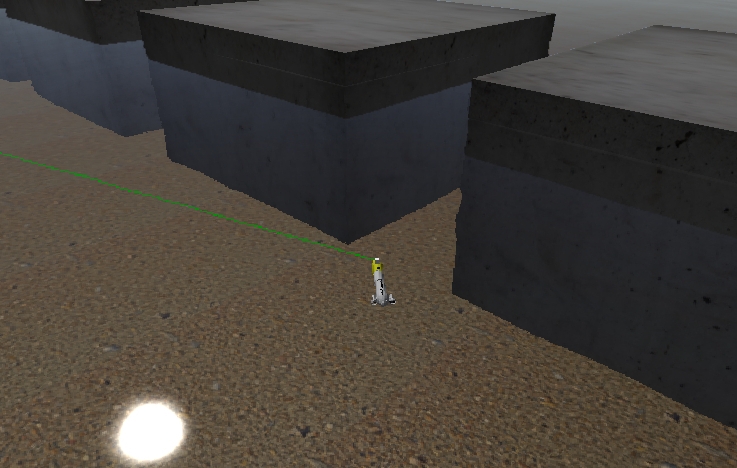
\includegraphics[width=.45\linewidth]{RRTstarPruning4}} \quad
    \subfloat[]
    {\label{fig:RRTstarPruning2}
    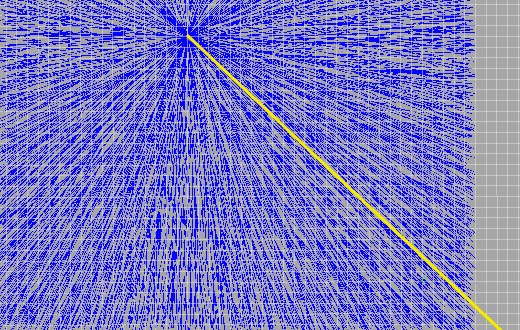
\includegraphics[width=.45\linewidth]{RRTstarPruning1}} \\
    \subfloat[]
    {\label{fig:RRTstarPruning3}
     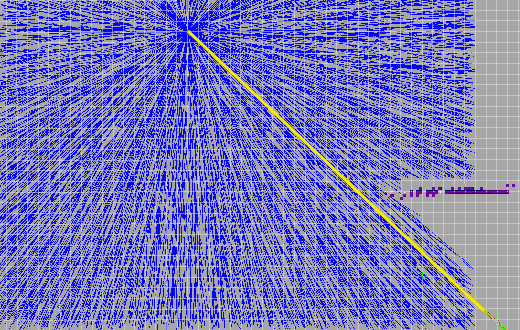
\includegraphics[width=.45\linewidth]{RRTstarPruning2}} \quad
    \subfloat[]
    {\label{fig:RRTstarPruning4}
    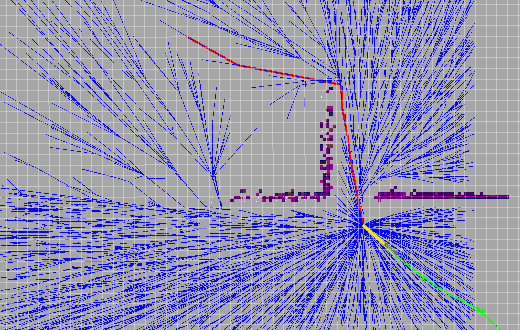
\includegraphics[width=.45\linewidth]{RRTstarPruning3}}
\caption[Sparus~II AUV conducting a mission in the simulated
breakwater structure using the pruning tree approach.]
{Sparus~II \ac{AUV} conducting a mission in the simulated breakwater structure
\protect\subref{fig:RRTstarPruning1}, where it incrementally maps the
environment \protect\subref{fig:RRTstarPruning2},
\protect\subref{fig:RRTstarPruning3} and (re)plans a collision-free path to the
goal \protect\subref{fig:RRTstarPruning4}. The tree of configurations is
presented in dark blue, the path to the goal in red, the path to the current
waypoint in yellow, and the vehicle's trajectory in green.}
\label{fig:RRTstarPruning}
\end{figure}

\subsubsection{Reuse of the Last Best Known Solution for Anytime Computation}

The previously explained approach used a tree of configurations that is
periodically traversed, checked and pruned as the vehicle moves and explores the
environment. The main objective was to preserve the information about
collision-free areas and known paths, while discarding those that become
invalid. One alternative for not conserving the whole tree, is to use the
\textit{last best known solution} as the remainder of the path calculated in the
previous planning cycle, which starts at the point that the vehicle will reach
at the next execution cycle (see
Fig.~\ref{fig:ReuseLastBestKnownSolutionState}). 

In this iterative and \textit{anytime} computation scheme, using the last
solution to start a new planning cycle implies not only a new valid solution
according to an updated map, but also one that is at least as optimal as the
previous one. This also permits to eliminate time-consuming pruning routines by
avoiding checking subtrees, in which many of their configurations have probably
become invalid because of the \textit{opportunistic state checking} explained
before.

\begin{figure}[htbp]
\myfloatalign
    \subfloat[]
    {\label{fig:ReuseLastBestKnownSolutionState1}
     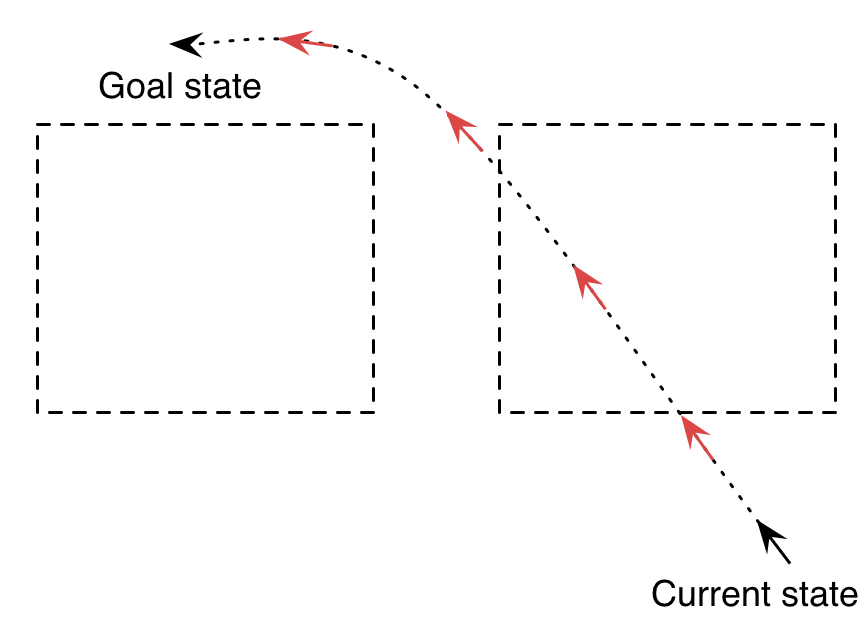
\includegraphics[width=.43\linewidth]{ReuseLastBestKnownSolutionState1}} \quad
    \subfloat[]
    {\label{fig:ReuseLastBestKnownSolutionState2}
    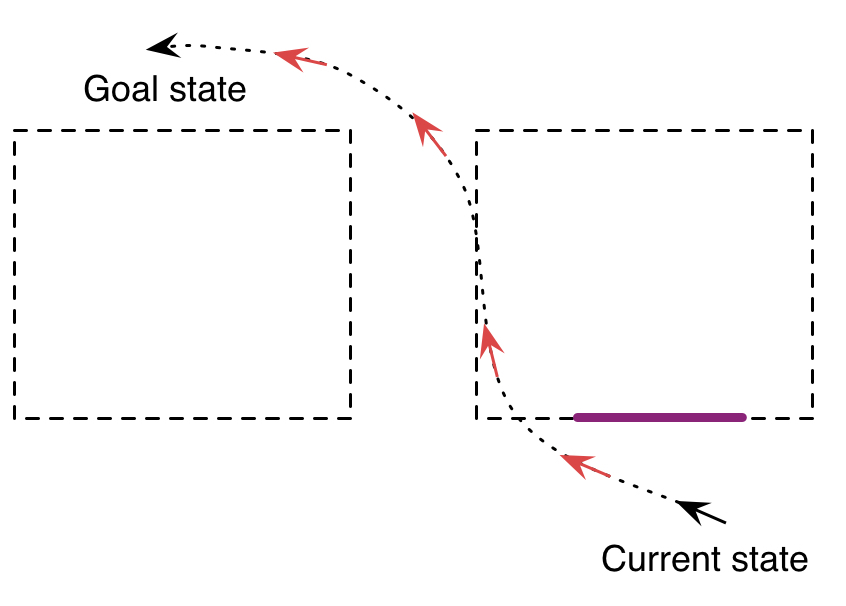
\includegraphics[width=.43\linewidth]{ReuseLastBestKnownSolutionState2}} \\
    \subfloat[]
    {\label{fig:ReuseLastBestKnownSolutionState3}
    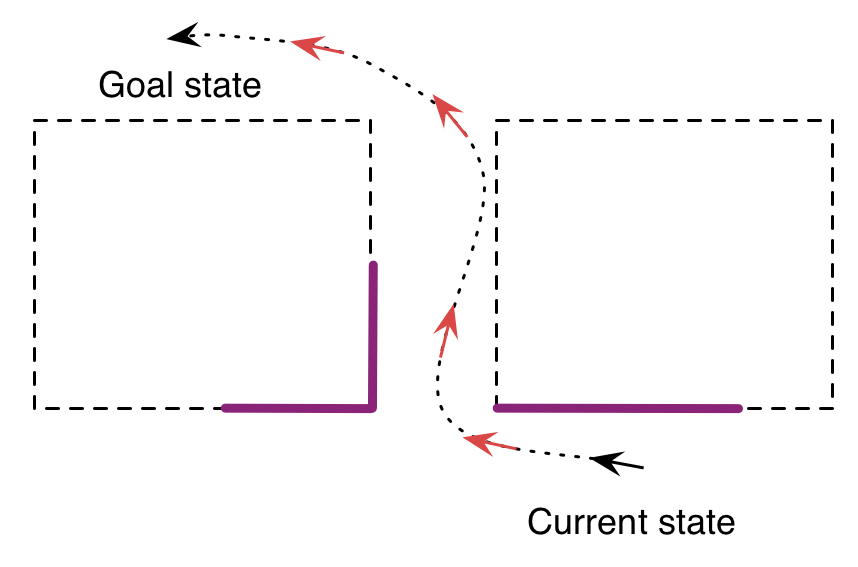
\includegraphics[width=.43\linewidth]{ReuseLastBestKnownSolutionState3}}
     \quad
    \subfloat[]
    {\label{fig:ReuseLastBestKnownSolutionState4}
    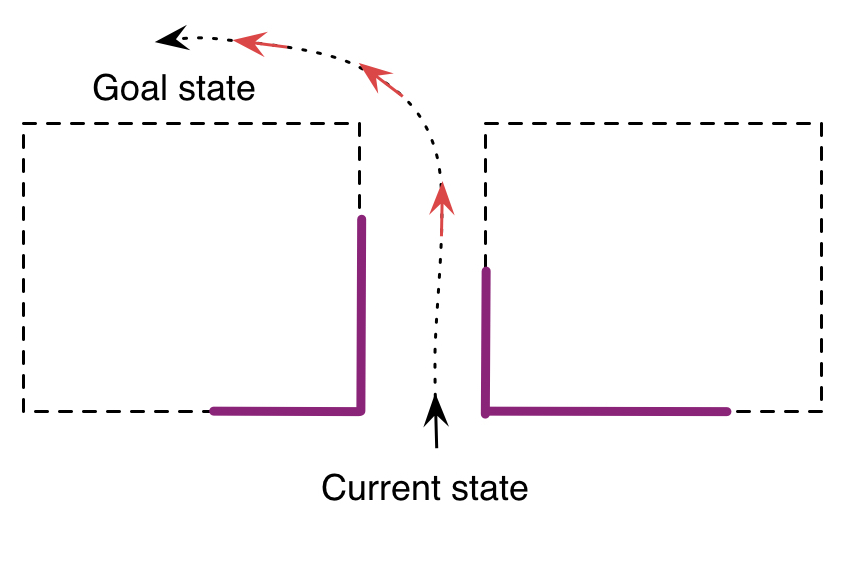
\includegraphics[width=.43\linewidth]{ReuseLastBestKnownSolutionState4}}
\caption[Reuse of the last best known solution.]
{Reuse of the last best known solution. This strategy allows reusing the
previous solution path for every new planning cycle, instead of checking and
pruning the whole tree. This guarantees having valid solutions that are at
least as good as the previous one.}
\label{fig:ReuseLastBestKnownSolutionState}
\end{figure}

\section{Pipeline for Online Planning Feasible and Safe Paths}
\label{sec:PipelineOnlPlanFeasSafePaths}

Previous sections have presented three new features: an optimization function
that combines collision risk and path length; a strategy to avoid unnecessary
and expensive state checking routines; and the reuse of the last best known
solution as a starting point for an anytime planning approach. These features
endow an \ac{AUV} with the capability to simultaneously map and plan feasible
and safe paths online through unexplored environments. In order to fully
understand how such characteristics work together,
Algorithm~\ref{alg:PlanningFramework} presents the execution pipeline to
incrementally solve a start-to-goal query. This pipeline has allowed conducting
autonomous missions for the intended \ac{AUV} applications. For this reason, the
newly proposed features represent the main contributions to the
\textit{planning} module presented in this chapter.

In Algorithm~\ref{alg:PlanningFramework}, the main input parameters to solve a
query are the start and goal configurations (position and orientation). To
initialize the incremental solving routine, the \ac{RRT*} algorithm is selected
as the planner that computes paths for a Dubins (or extended \ac{3D} Dubins)
vehicle, set an empty list as the \textit{last best known solution}, and define
$q_{new\_start}$ as the starting configuration that will change as the vehicle
conduct the mission
(lines~\ref{lin_alg:dubins_st_sp}-\ref{lin_alg:initial_start}).
To incrementally find a path to the goal (line~\ref{lin_alg:main_loop}), a main
loop requests an updated version of the map (Octomap,
lines~\ref{lin_alg:ReqUpdatedMap}-\ref{lin_alg:SetUpdatedMap}), informs the
planner to start from \textit{last best known solution}
(line~\ref{lin_alg:start_from}), uses the planner to find or improve the path
(line~\ref{lin_alg:solve_query}), and gets the solution
(line~\ref{lin_alg:get_solution}). At this point, the planner has provided a
valid path that must be as optimal as the previous one, except that it has
produced a longer but safer path. Before concluding a planning cycle, the
incremental solving routine checks if a replanning maneuver has been requested.
This would imply that the \textit{mission handler} has detected that the path
from the current configuration to the last \ac{WP} sent to the \ac{AUV}
controllers is not feasible, and might lead the vehicle to a collision, thus
requiring that a new path should be found from the current configuration (see
lines~\ref{lin_alg:replan_first}-\ref{lin_alg:replan_last}).
Finally, if a new \ac{WP} is required, the last $q_{new\_start}$ will be sent to
the \textit{mission handler}
(lines~\ref{lin_alg:req_new_wp1}-\ref{lin_alg:req_new_wp2}).

It is important to note that even if the previous (\textit{last best known})
solution is not in collision with an updated version of the map, the
\textit{planning} module will reuse it as a starting point
(line~\ref{lin_alg:start_from}), in order to attempt to improve such existing
solution during a new planning cycle (lines~\ref{lin_alg:solve_query}
and~\ref{lin_alg:get_solution}).

\begin{algorithm}[htbp]
	\DontPrintSemicolon
	\SetKwFunction{RRTstar}{RRT*}
	\SetKwFunction{reqUpdatedMap}{reqUpdatedMap}
	\SetKwFunction{updateMap}{updateMap}
	\SetKwFunction{startFrom}{startFrom}
	\SetKwFunction{solve}{solve}
	\SetKwFunction{getSolution}{getSolution}
	\SetKwFunction{sendWP}{sendWP}
	\SetKwFunction{pop}{pop}
	\SetKwFunction{getCurrentConf}{getCurrentConf}

	\KwIn{\\ 
	$q_{start}$: Start configuration.\\
	$q_{goal}$: Goal configuration.}
% 	\KwOut{\\ $T$: an RRT that contains the collision-free path (if found).}

 	\Begin{
 		$planner\leftarrow\RRTstar{}$\;\label{lin_alg:dubins_st_sp}
 		$last\_best\_known\_solution\leftarrow\{\}$\;\label{lin_alg:initial_solution}
 		$q_{new\_start}\leftarrow q_{start}$\;\label{lin_alg:initial_start}
 		\While{not $stop\_condition$}{\label{lin_alg:main_loop}
 			$map \leftarrow$\reqUpdatedMap{}\;\label{lin_alg:ReqUpdatedMap}
 			$planner.\updateMap{map}$\;\label{lin_alg:SetUpdatedMap}
 			$planner.\startFrom{last\_best\_known\_solution}$\;\label{lin_alg:start_from}
 			$planner.$\solve{$q_{new\_start},q_{goal}$}\;\label{lin_alg:solve_query}
 			$last\_best\_known\_solution\leftarrow
 			planner.$\getSolution{}\;\label{lin_alg:get_solution}
 			\If{$replanning\_requested$} {\label{lin_alg:replan_first}
 				$q_{new\_start}\leftarrow \getCurrentConf{}$\;
 				$last\_best\_known\_solution\leftarrow\{\}$\;\label{lin_alg:replan_last}
 				}
  			\ElseIf{$new\_waypoint\_requested$} {\label{lin_alg:req_new_wp1}
  				\sendWP{$last\_best\_known\_solution$.\pop{}}\;\label{lin_alg:req_new_wp2}
  			}
 		}
 	}
 \caption{incSolveStart2Goal$\left(q_{start},q_{goal}\right)$}
 \label{alg:PlanningFramework}
\end{algorithm}

\section{Results}
\label{sec:PlanningOnlineResults}

In order to validate the proposed path/motion planning framework, this section
presents simulation and real-world trials of the Sparus~II \ac{AUV} conducting
autonomous missions in the breakwater structure scenario. This structure is
located in the external and open area of a harbor, and it is composed
 of a series of concrete blocks of $14.5m$ long and $12m$ width, separated by a
four-meter gap with an average depth of $7m$ (see
Fig.~\ref{fig:SantFeliu_Blocks}). In this scenario, start and goal
configurations were located in opposite sides, so that the Sparus~II \ac{AUV}
had to move amidst the concrete blocks. All queries were defined to conduct
missions at a constant depth, thus the motion was restricted to a \ac{2D} task.


\begin{figure}[htbp]
	\centering
	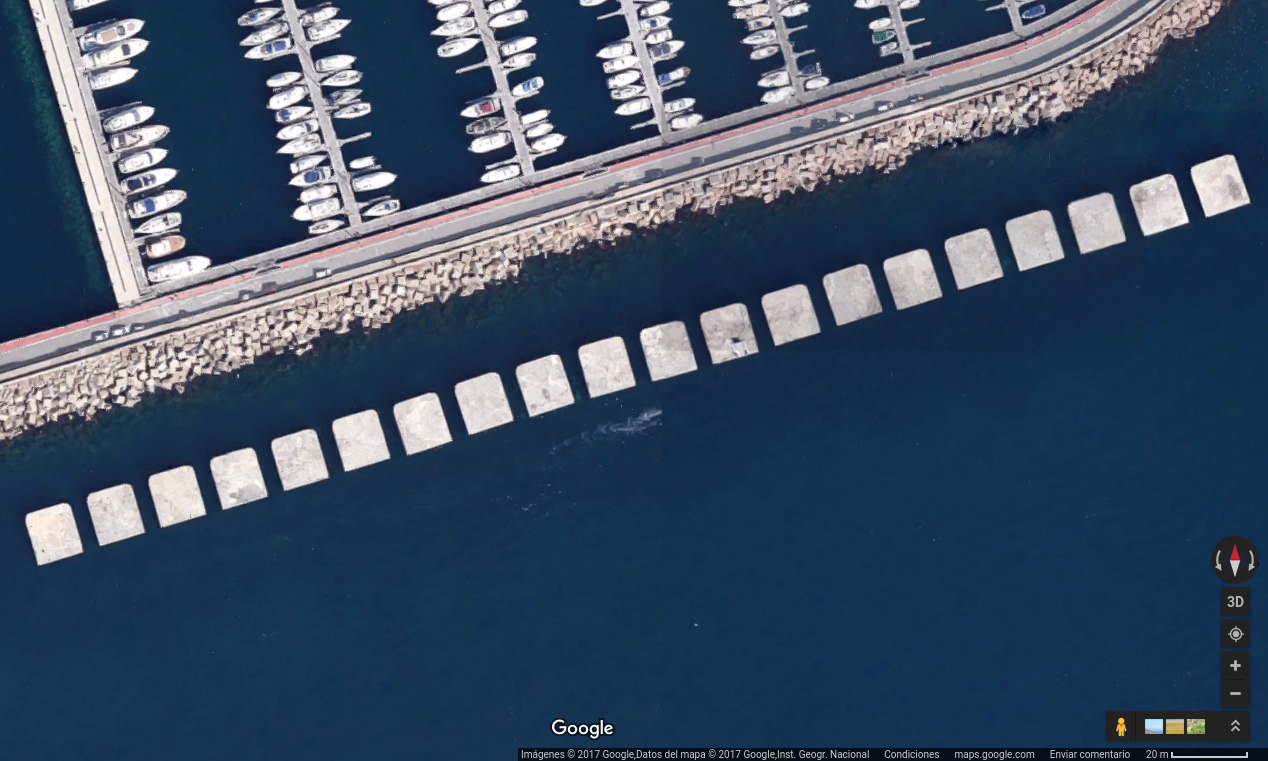
\includegraphics[width=.85\linewidth]{BreakwaterStructureGoogleMaps} 
\caption[Satellite image of the breakwater structure that is composed of a
series of concrete blocks.] 
{Breakwater structure composed of a series of concrete blocks ($14.5m$ long and
$12m$ width, separated by a four-meter gap) in Sant Feliu de Gu\'ixols in
(Spain). Image credit: Map data \copyright 2017 Google.}
\label{fig:SantFeliu_Blocks}
\end{figure}

For these tests, the vehicle was equipped with a mechanically-scanning profiling
sonar to perceive and detect the surroundings. The sonar was located to cover a
scan sector in the horizontal plane along the vehicle's direction of motion.
From the software perspective, the Sparus~II used the
\ac{COLA2}~\cite{Palomeras2012}, a control architecture fully integrated with
the \ac{ROS}. This software architecture also makes use of the \ac{OMPL} that
offers a convenient framework that can be adapted to specific planning
problems~\cite{Sucan2012}. Further details about the vehicle hardware and
software characteristics can be found in Appendix~\ref{appx:exp_platform}.

\subsection{Comparison of Risk Functions}

Before evaluating the framework's capabilities over unexplored environments,
this section firstly assesses and establishes the best alternative to estimate the
risk associated with a path. This analysis is done over a fully known and mapped
scenario. Once this has been determined, tests over an unexplored environment
prove the advantages of using the \textit{opportunistic state check} strategy.
Then, with this strategy, additional tests compares both the
\textit{pruning} tree and the \textit{reuse of the last best known solution}
approaches, thus allowing to demonstrate the latter one is the most efficient
alternative for reaching an anytime computation approach.

\subsubsection{Evaluation of the Risk Functions over Fully Mapped Environments}

For these initial tests, an Octomap of the surroundings was assumed to be
available \textit{a priori}. Over this map, different start-to-goal queries were
solved by using the alternatives to estimate the risk presented in
Sec.~\ref{sec:RiskFunctions}. Figure~\ref{fig:CompareRiskFunctionsTasks} depicts
some examples of the solutions paths obtained. It can be observed how the path
maintains a safe distance from nearby obstacles (areas in purple), in contrast
to what occurs when only path length criterion was considered (see
Fig.~\ref{fig:GeomRRTstarDubPathLeng_Rviz}).

\begin{figure}[htbp]
\myfloatalign
    \subfloat[Task1]
    {\label{fig:GeomRRTstarDubRiskFunctT1}
     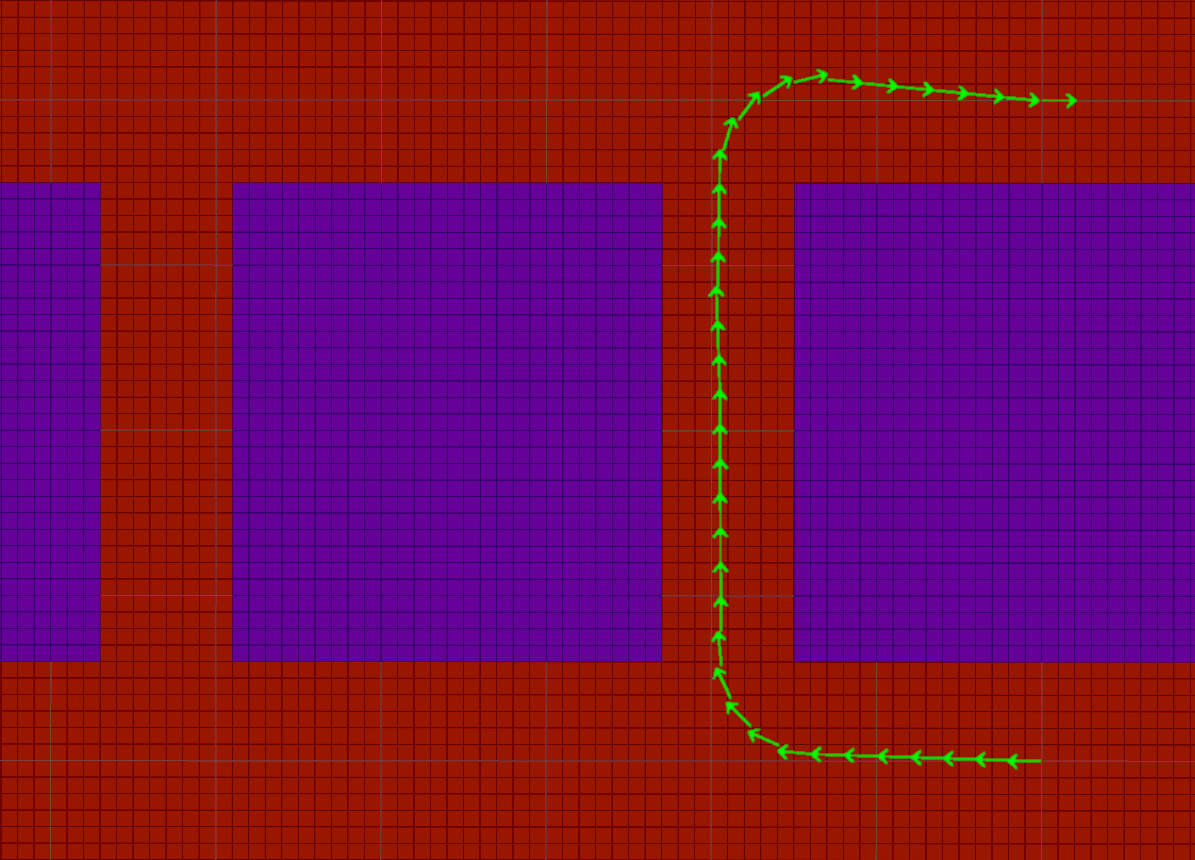
\includegraphics[width=.45\linewidth]{GeomRRTstarDubRiskFunctT1}} \quad
    \subfloat[Task2]
    {\label{fig:GeomRRTstarDubRiskFunctT2}
    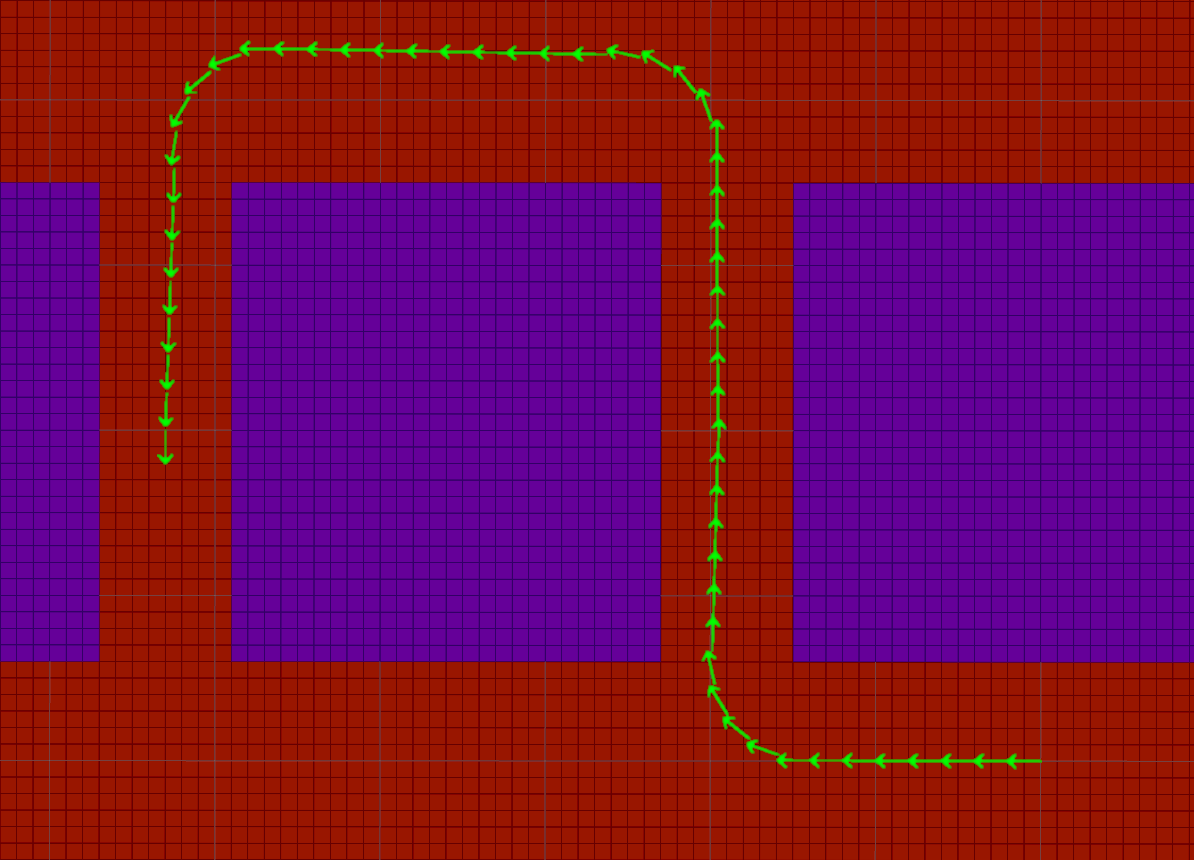
\includegraphics[width=.45\linewidth]{GeomRRTstarDubRiskFunctT2}}
\caption[Start-to-goal queries' solutions using an RRT* algorithm with Dubins
curves and risk functions. The solution paths maintain a safe distance from nearby
obstacles.]
{Start-to-goal queries' solutions using an \ac{RRT*} algorithm with Dubins
curves and risk functions. The solution paths maintain a safe distance from nearby
obstacles (areas in purple).}
\label{fig:CompareRiskFunctionsTasks}
\end{figure}

Although all of the proposed approaches to estimate risk of the path can
generate similar results, their associated computation times differ
considerably. Figure~\ref{fig:CompareRiskFunctions} presents the average
computation time required to solve $Task1$ and $Task2$
(Fig.~\ref{fig:CompareRiskFunctionsTasks}) by each approach. It can be observed
that using only the \textit{path length} is clearly the least expensive method,
while \textit{path length + clearance} and \textit{risk vectors} are the most
and least expensive, respectively, when including the risk of the path. For
this reason, the best alternative when dealing with explored (mapped)
environments is the \textit{risk vectors} approach.

\begin{figure}[htbp]
	\centering
	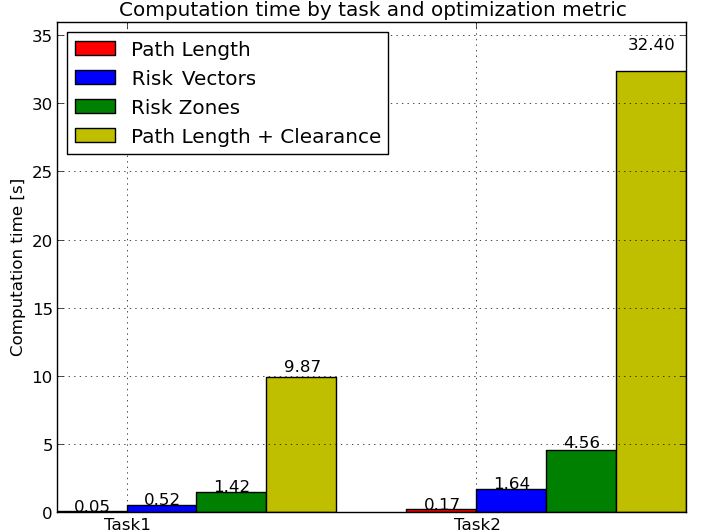
\includegraphics[width=.8\linewidth]{CompareRiskFunctions} 
\caption[Average computation time required by the planner when using different
alternatives to estimate the risk associated with a path.] 
{Average computation time, over 20 runs, required to solve $Task1$ and $Task2$
(Fig.~\ref{fig:CompareRiskFunctionsTasks}) using different approaches to include
risk of the path as the optimization criterion.}
\label{fig:CompareRiskFunctions}
\end{figure}

\subsubsection{Evaluation of the Risk Functions over Unknown Environments} 

From Fig.~\ref{fig:CompareRiskFunctions}, it can be concluded that the best
computational alternative to include the risk associated with a path is the
\textit{risk vectors} approach. However, when dealing with unexplored
environments, \ie exploring while mapping incrementally, this approach may cope
with situations in which partial information of the environment does not permit
to estimate correctly the risk. In turning maneuvers, for instance, if an
obstacle is located in the lateral motion direction, and it is not completely
represented in the map so that the \textit{risk vectors} does not coincide with
the available partial information, this approach will indicate the configuration
as safe, while the \textit{risk zones} will estimate correctly the risk. For
this reason, the best alternative when dealing with unexplored (unknown)
environments is the \textit{risk zones} approach.

\subsection{Opportunistic State Checking and its Benefits}

Although planning feasible and safe paths using \textit{risk zones} is
considerably faster than calculating clearance explicitly (see
Fig.~\ref{fig:CompareRiskFunctions}), having calculation times in the order of
seconds may become into a limitation when coping with online computation
limitations. Section~\ref{sec:OportStateCheck} introduced the
\textit{opportunistic state checking} strategy as one of the mechanisms that can
contribute to overcome this situation. To validate its efficiency, a
start-to-goal query was solved and simulated multiple times, but now without
assuming any previous map of the breakwater structure scenario (see
Fig.~\ref{fig:MappingPlanningOpportRisk}).

\begin{figure}[htbp]
\myfloatalign
    \subfloat[]
    {\label{fig:Sparus2-InitialPos-UWSim}
     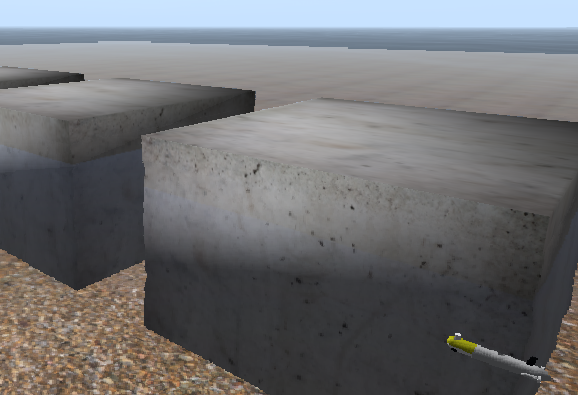
\includegraphics[width=.45\linewidth]{Sparus2-InitialPos-UWSim}} \quad
    \subfloat[]
    {\label{fig:MappingPlanningOpportRisk1}
    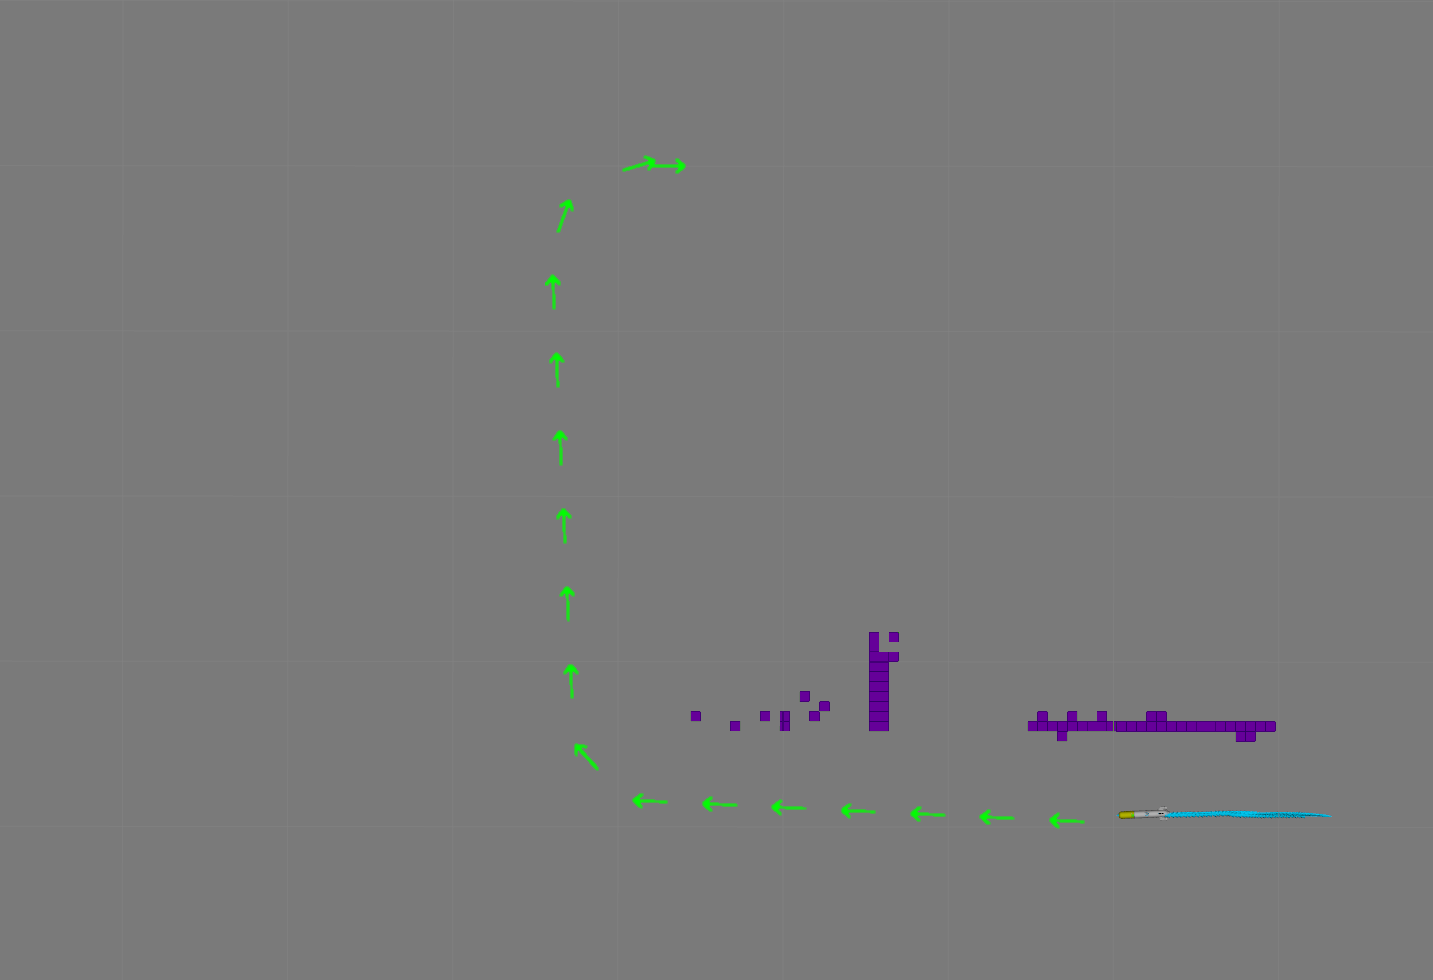
\includegraphics[width=.45\linewidth]{MappingPlanningOpportRisk1}} \\
    \subfloat[]
    {\label{fig:MappingPlanningOpportRisk2}
    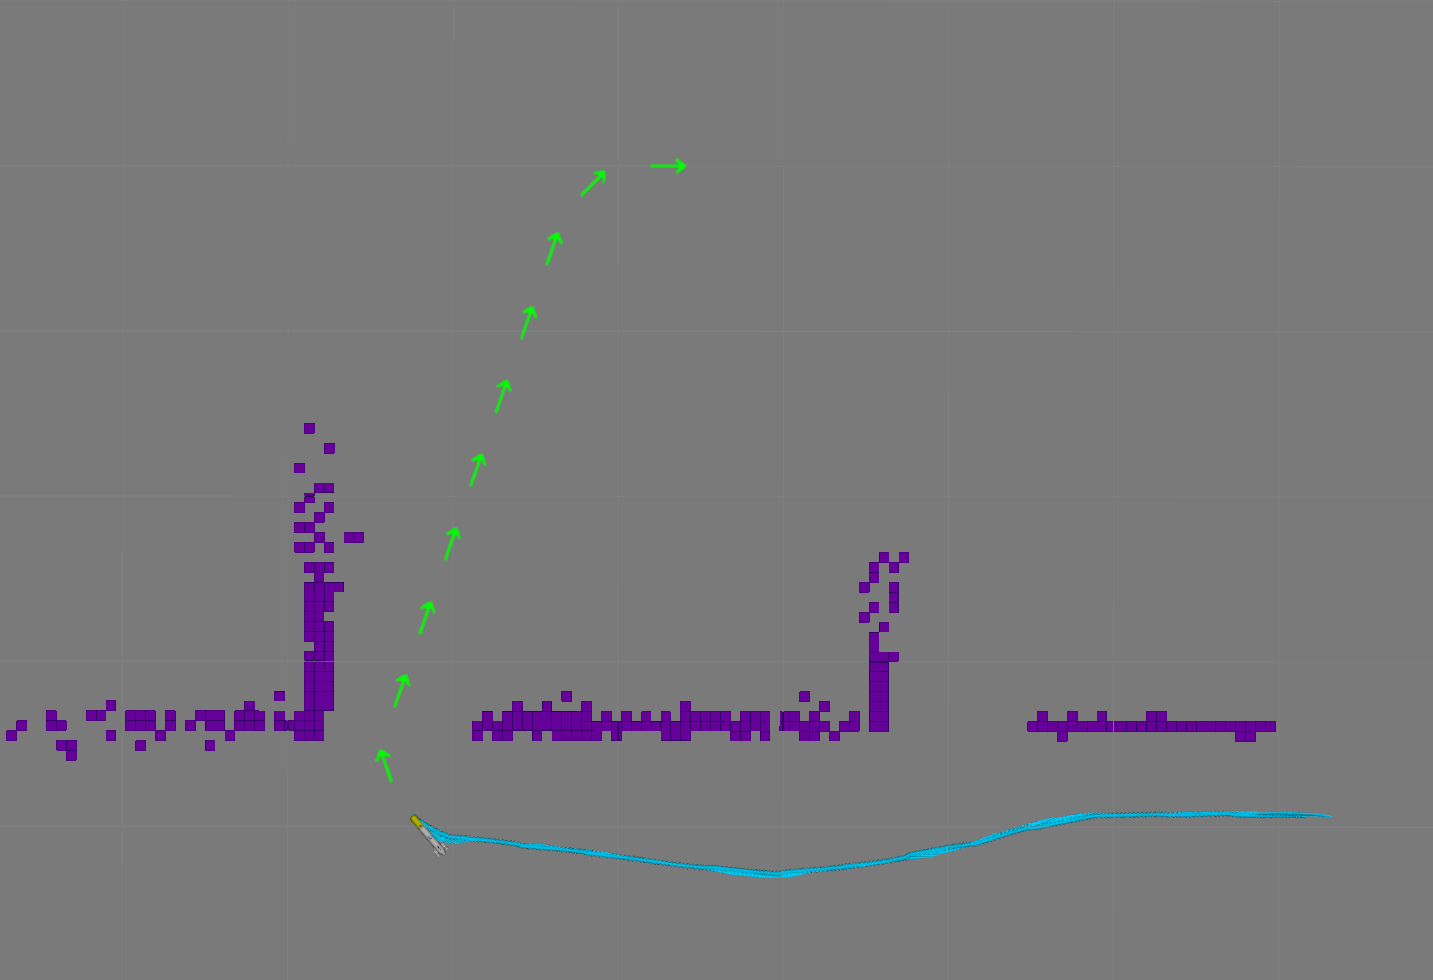
\includegraphics[width=.45\linewidth]{MappingPlanningOpportRisk2}}
     \quad
    \subfloat[]
    {\label{fig:MappingPlanningOpportRisk3}
    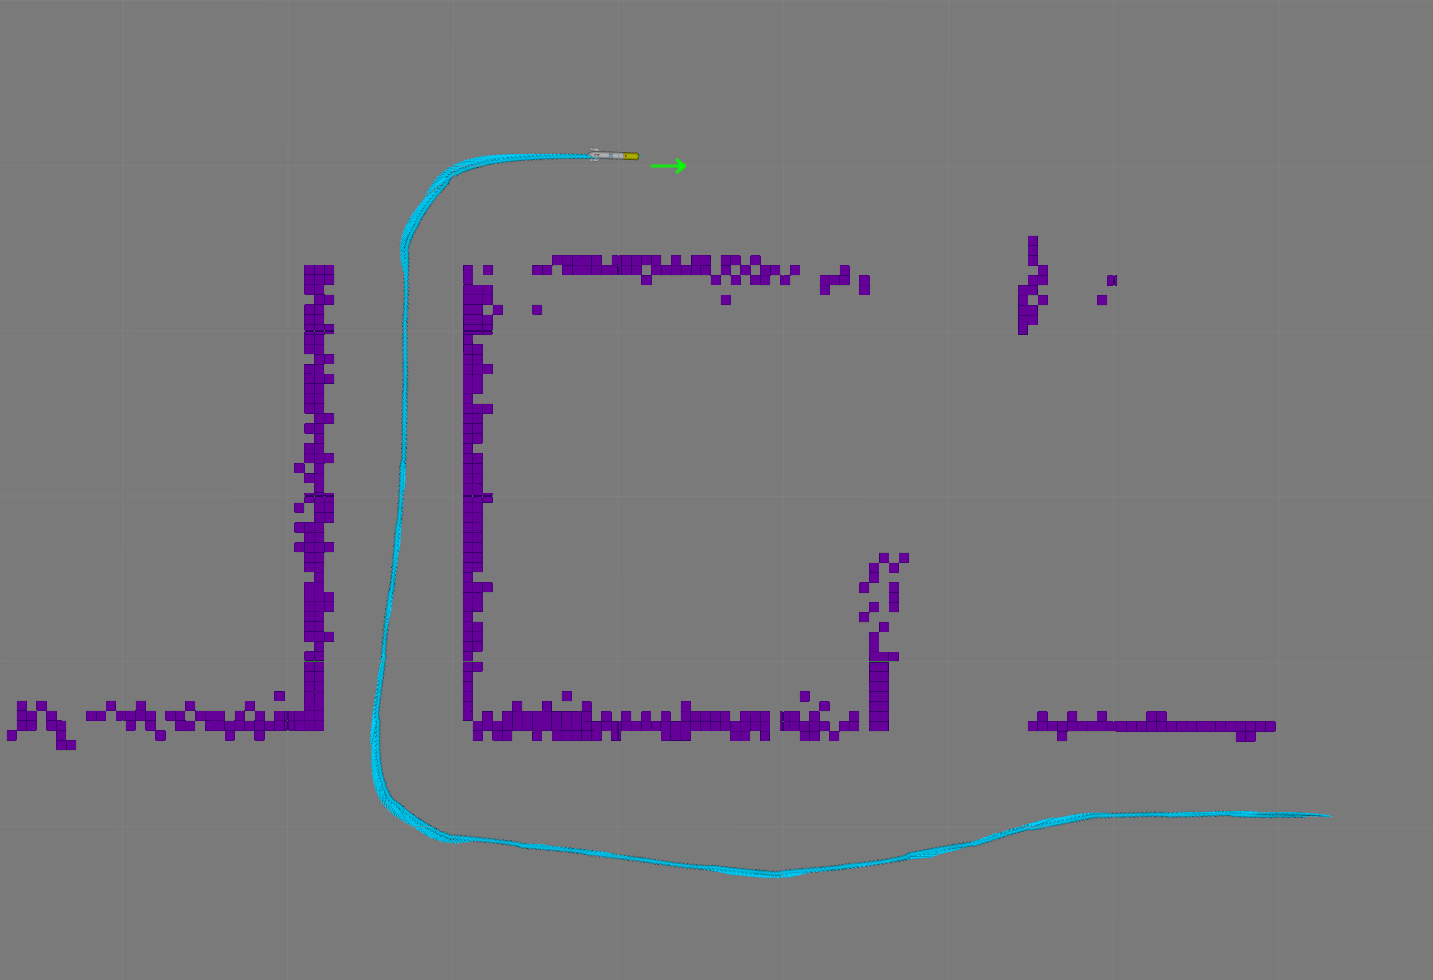
\includegraphics[width=.45\linewidth]{MappingPlanningOpportRisk3}}
\caption[Sparus~II solving a start-to-goal query in an equivalent virtual
scenario of the breakwater structure without an initial map.]
{\protect\subref{fig:Sparus2-InitialPos-UWSim} Sparus~II initial position for
different start-to-goal queries in an equivalent virtual scenario of the
breakwater structure.~\protect\subref{fig:MappingPlanningOpportRisk1}~Sparus~II
starts a mission by submerging to a specified depth. It then maps and solves a
start-to-goal query simultaneously.
\protect\subref{fig:MappingPlanningOpportRisk2} Equipped with a scanning
profiler, it incrementally builds a representation of the environment, while
continuously reshaping the solution
path,~\protect\subref{fig:MappingPlanningOpportRisk3} to finally approach to the
specified goal configuration.}
\label{fig:MappingPlanningOpportRisk}
\end{figure}

The solutions for the query presented in
Fig.~\ref{fig:MappingPlanningOpportRisk} were obtained with and without using
the \textit{opportunistic state checking} strategy. Albeit in both cases the
framework succeeded in conducting the task,
Fig.~\ref{fig:CompareCompTimeOpportRiskCheck} demonstrates that without it
almost $80\%$ of the total computation time is dedicated to risk checking
routines over the whole mission. In the opposite scenario, \ie using
\textit{opportunistic state checking}, its associated computation time increases
as the environment is progressively explored, but even so, it does not consume
such a percentage of computation time, not even at the end of the mission. This
is especially noticeable when a mission does not require exploring and mapping
completely the environment. Therefore, the use of the proposed mechanism affects
not only the time required to find a solution, since it permits a better tree
expansion (\ie more states, see Fig.~\ref{fig:CompareNodesOpportRiskCheck}), but
also improves the workspace exploration and the path quality.
%  given by the
% asymptotic optimality of the algorithm.

\begin{figure}[htbp]
\myfloatalign
    \subfloat[]
    {\label{fig:CompareCompTimeOpportRiskCheck}
     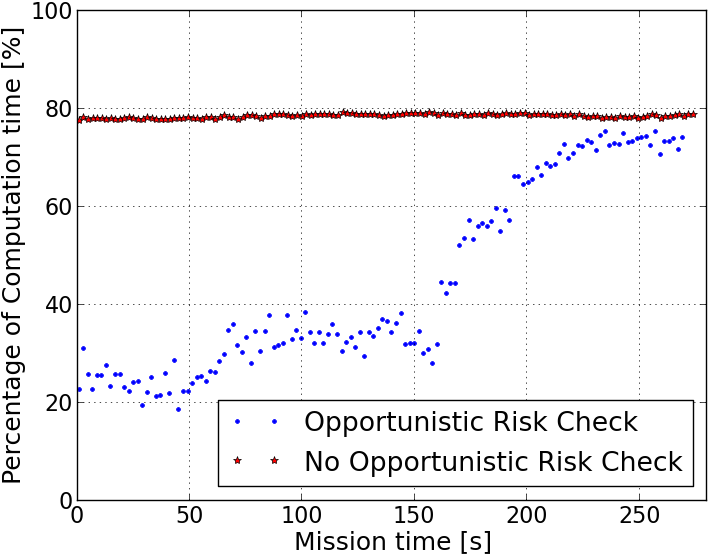
\includegraphics[width=.45\linewidth]{CompareCompTimeOpportRiskCheck}} \quad
    \subfloat[]
    {\label{fig:CompareNodesOpportRiskCheck}
    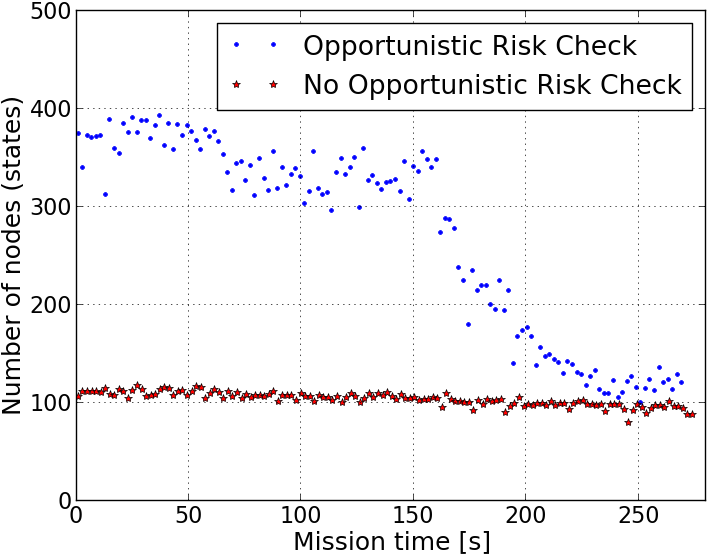
\includegraphics[width=.45\linewidth]{CompareNodesOpportRiskCheck}}
\caption[Incidence of \textit{Opportunistic State Checking} approach when
solving a start-to-goal query.]
{Incidence of \textit{Opportunistic State Checking} approach when
solving query presented in Fig.~\ref{fig:MappingPlanningOpportRisk}.
\protect\subref{fig:CompareCompTimeOpportRiskCheck} if configurations located in
undiscovered areas are not assumed as safe, risk checking routines require
almost $80\%$ of computation time during the whole mission. Otherwise, it will
increase progressively as the environment is explored.
\protect\subref{fig:CompareNodesOpportRiskCheck} consequently, if a high
percentage of computing power is dedicated to risk checking, the number of tree
nodes (states) will remain low during the whole mission, thus limiting the tree
expansion and path quality.}
\label{fig:CompareOpportRiskCheck}
\end{figure}

\subsection{Anytime Computation for Solving Start-to-goal Queries in Unexplored
Environments}

Section~\ref{sec:ReuseLastBestKnownSol} presented a \textit{pruning} tree scheme
and the \textit{reuse of the last best known solution}. Both are alternative
replanning approaches to make the framework capable of providing valid solutions
at \textit{anytime}. In order to prove the latter one is the best option, the
execution pipeline presented in Sec.~\ref{sec:PipelineOnlPlanFeasSafePaths} has
been used with both approaches to run different simulations and real-world
in-water trials.

\subsubsection{Simulation Results} 

Two different simulated scenarios were used to compare the \textit{anytime}
computation approaches. The first of them is the breakwater structure mentioned
in previous sections (see
Figs.~\ref{fig:SantFeliuBlocksOctomap},~\ref{fig:SantFeliu_Blocks}). Over this
scenario, two different start-to-goal queries were tested (see
Fig.~\ref{fig:TestsBlocksScenario}). After executing $10$ times these missions,
it was observed that the number of successful attempts is greater and the mean
of replanning maneuvers (over the total successful missions) is smaller when
\textit{reusing the last best known solution} with \textit{opportunistic state
checking}, than those obtained with the \textit{pruning} tree scheme (see
Tables~\ref{table:TestsBlocksScenario} and \ref{table:TestsCanyonScenario}).
Such replanning maneuvers correspond to situations where the calculated path was
unfeasible, thus requiring a new valid path.

\begin{figure}[htbp]
\myfloatalign
    \subfloat[Task1, pruning the tree]
    {\label{fig:BlocksScenarioTest1OldFram}
     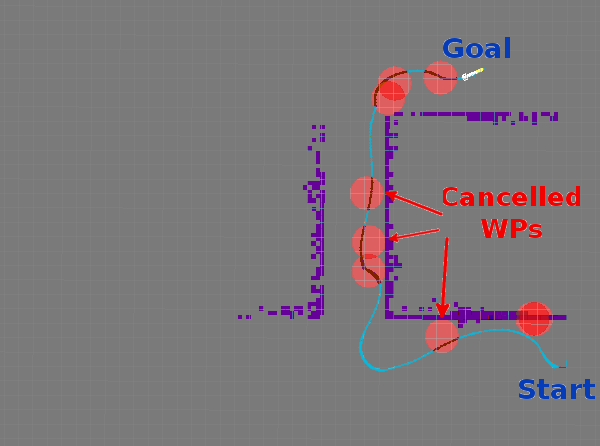
\includegraphics[width=.4\linewidth]{BlocksScenarioTest1OldFram}} \quad
    \subfloat[Task2, pruning the tree]
    {\label{fig:BlocksScenarioTest2OldFram}
    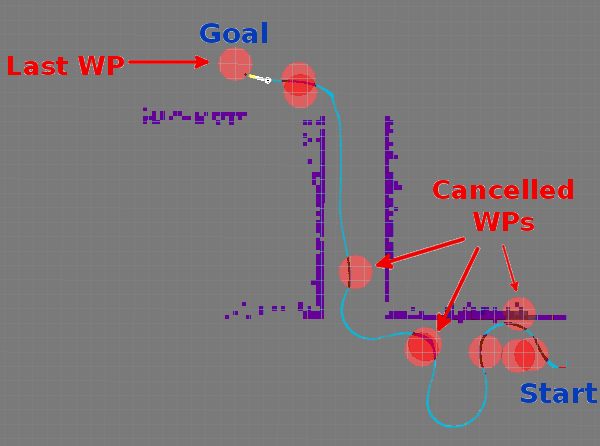
\includegraphics[width=.4\linewidth]{BlocksScenarioTest2OldFram}} \\
    \subfloat[Task1, reuse last best solution]
    {\label{fig:BlocksScenarioTest1NewFram}
    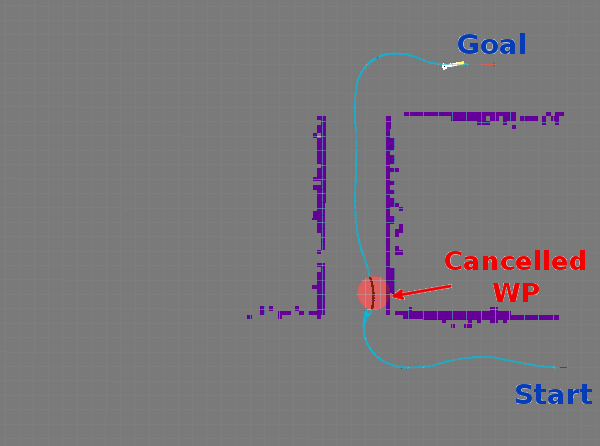
\includegraphics[width=.4\linewidth]{BlocksScenarioTest1NewFram}}
     \quad
    \subfloat[Task2, reuse last best solution]
    {\label{fig:BlocksScenarioTest2NewFram}
    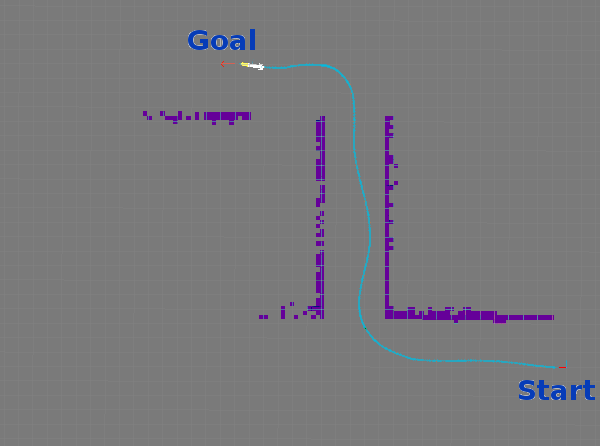
\includegraphics[width=.4\linewidth]{BlocksScenarioTest2NewFram}}
\caption[Comparison of the \textit{anytime} computation approaches when solving
start-to-goal queries without an initial map.]
{Comparison of the \textit{anytime} computation approaches when solving
start-to-goal queries with the \textit{pruning-tree} scheme and the
\textit{reuse of the last best known solution} approaches. The number of
replanning maneuvers are equivalent to the number of cancelled \acp{WP} (circles
in red).}
\label{fig:TestsBlocksScenario}
\end{figure}

The second test scenario resembles a natural environment composed of rocky
formations, which create an underwater canyon (see
Figs.~\ref{fig:RocksScenarioUWSim1},~\ref{fig:RocksScenarioUWSim2}). Over it,
one start-to-goal query was defined in a way that the vehicle was required to
travel through the canyon (see
Figs.~\ref{fig:RocksScenarioTest1OldFram},~\ref{fig:RocksScenarioTest1NewFram}).
Once again, it was observed that the number of successful attempts is greater
and the mean of replanning maneuvers is smaller in the case of \textit{reusing
the last best known solution} with \textit{opportunistic state checking} (see
Tables~\ref{table:TestsBlocksScenario} and \ref{table:TestsCanyonScenario}).

\begin{figure}[htbp]
\myfloatalign
    \subfloat[Sea rocks scenario]
    {\label{fig:RocksScenarioUWSim1}
     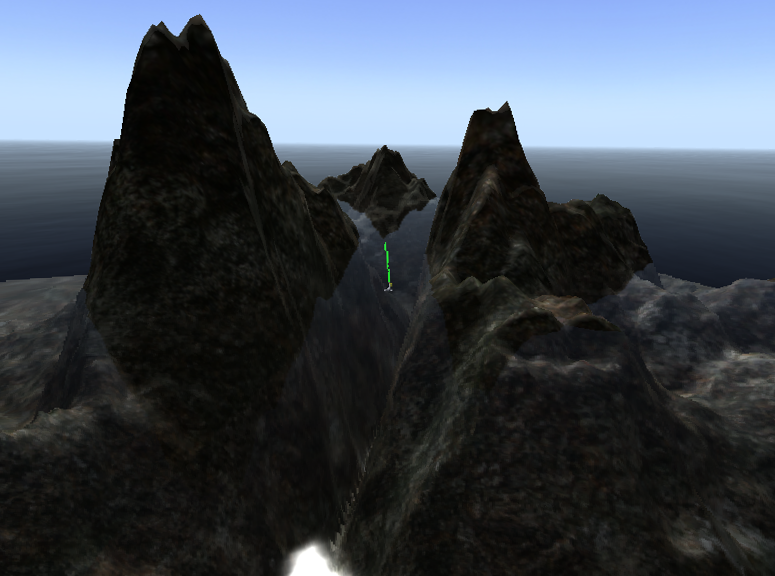
\includegraphics[width=.45\linewidth]{RocksScenarioUWSim1}} \quad
    \subfloat[Navigating through the canyon]
    {\label{fig:RocksScenarioUWSim2}
    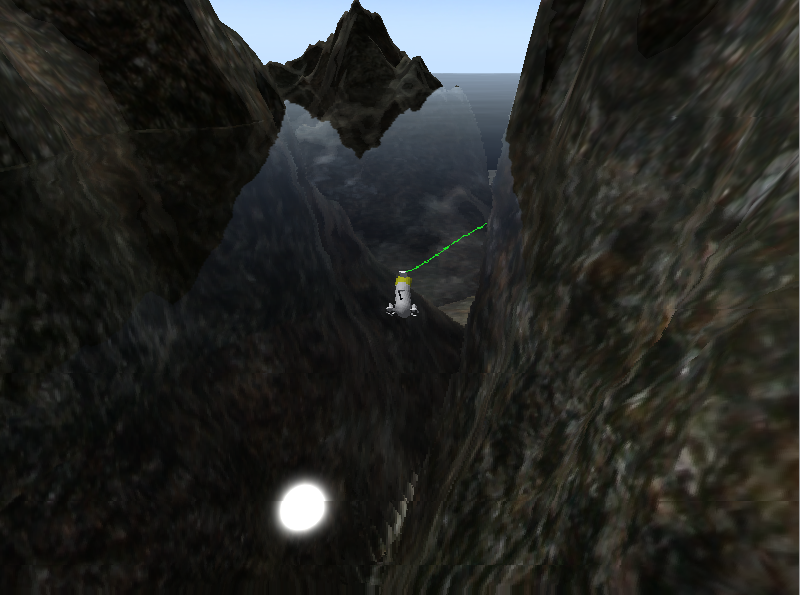
\includegraphics[width=.45\linewidth]{RocksScenarioUWSim2}} \\
    \subfloat[Pruning the tree]
    {\label{fig:RocksScenarioTest1OldFram}
    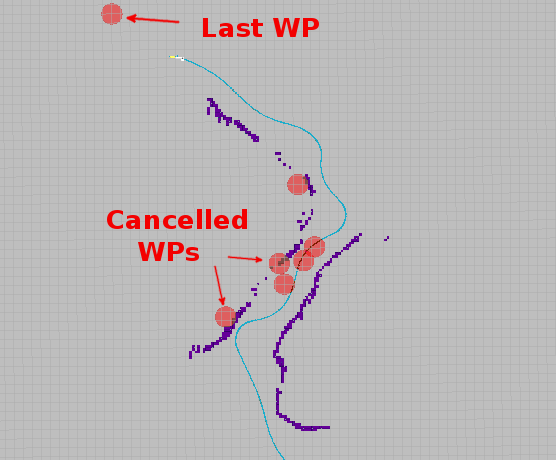
\includegraphics[width=.45\linewidth]{RocksScenarioTest1OldFram}}
     \quad
    \subfloat[Reuse last best solution]
    {\label{fig:RocksScenarioTest1NewFram}
    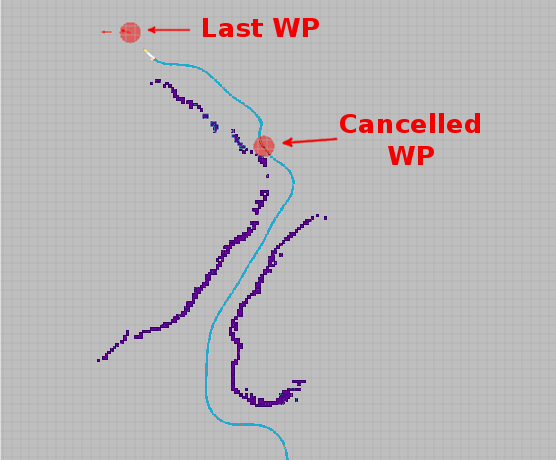
\includegraphics[width=.45\linewidth]{RocksScenarioTest1NewFram}}
\caption[Comparison of the \textit{anytime} computation approaches when solving
start-to-goal queries without an initial map over a simulated natural-like
environment.]
{Comparison of the \textit{anytime} computation approaches when solving
start-to-goal queries with the \textit{pruning-tree} scheme and the
\textit{reuse of the last best known solution} approaches. The simulated
scenario resembles a natural-like environment. The number of replanning
maneuvers are equivalent to the number of cancelled
\acp{WP} (circles in red).}
\label{fig:TestsRocksScenario}
\end{figure}


%\begin{landscape}

\begin{table}[htbp]
\begin{center}
\begin{tabular}{c|c|c|c|c|} 
\cline{2-5} & \multicolumn{4}{ c| }{Virtual Scenario1: Breakwater Structure (Fig.~\ref{fig:TestsBlocksScenario})} \\
\cline{2-5} & \multicolumn{2}{ c| }{Task1 (10 attempts)} & \multicolumn{2}{ c| }{Task 2 (10 attempts)} \\
\cline{2-5} & \# Successful & Mean replan. & \# Successful & Mean replan.\\
            & attempts      & maneuvers       & attempts      & maneuvers \\
\cline{1-5} \multicolumn{1}{ |c| }{\makecell{Pruning \\Tree}} & $7$ & $8.85$ & $7$ & $6.42$ \\
\cline{1-5} \multicolumn{1}{ |c| }{\makecell{Reuse \\Last Sol.}} & $10$ & $0.3$
& $9$ & $0.1$ \\
\cline{1-5} 
\end{tabular}
\end{center}
\caption[Comparison of the \textit{anytime} computation approaches when solving
start-to-goal queries without an initial map. The test scenario was a
simulated version of a breakwater structure .]
{Comparison of solving the task shown in Fig.~\ref{fig:TestsBlocksScenario} 
using \textit{pruning-tree} scheme and the \textit{reuse of the last best known
solution}. The second one proves to be the best alternative with:
1) the increase in the number of successful attempts, 2) the decrease of the
mean of replanning maneuvers over the total successful missions. This latter
implies that the vehicle had to deal with less risky situations, since a
replanning maneuver supposes that the vehicle was being led to a possible
collision.}
\label{table:TestsBlocksScenario}
\end{table}


\begin{table}[htbp]
\begin{center}
\begin{tabular}{c|c|c|} 
\cline{2-3} & \multicolumn{2}{ c| }{Virtual Scenario2: Sea Rocks (Fig.~\ref{fig:TestsRocksScenario})} \\
\cline{2-3} & \multicolumn{2}{ c| }{Task 3 (10 attempts)} \\
\cline{2-3} & \# Successful & Mean of replan. \\
            & attempts & maneuvers \\
\cline{1-3} \multicolumn{1}{ |c| }{Pruning Tree} & $6$ & $6.6$ \\
\cline{1-3} \multicolumn{1}{ |c| }{Reuse Last Sol.} & $7$ & $1.14$\\
\cline{1-3} 
\end{tabular}
\end{center}
\caption[Comparison of the \textit{anytime} computation approaches when solving
start-to-goal queries without an initial map. The test scenario was a simulated
natural-like environment.]
{Comparison of solving the task shown in Fig.\ref{fig:TestsRocksScenario} using
\textit{pruning-tree} scheme and the \textit{reuse of the last best known
solution}. As shown also in Table~\ref{table:TestsBlocksScenario}, reusing the
last best solution proves to be the best alternative.}
\label{table:TestsCanyonScenario}
\end{table}

%\end{landscape}

\subsubsection{Real-world Results}

After testing the planning framework in simulation, in-water trials were
conducted in the real-world breakwater structure scenario (see
Figs.~\ref{fig:SantFeliuBlocksOctomap},~\ref{fig:SantFeliu_Blocks}). The
Sparus~II \ac{AUV} performed the autonomous missions with a constant surge speed
$u=0.5m/s$ and a maximum turning rate $r_{max}=0.3rad/s$.
Figure~\ref{fig:BlocksRealWorldTests} presents the \ac{AUV} trajectory after
conducting one of such missions, which consisted in solving a start-to-goal
query that required the vehicle to navigate between two concrete blocks of the
breakwater structure. Here again both approaches, \ie the one using a tree
\textit{prunning} scheme and the one \textit{reusing the last best known
solution} with \textit{opportunistic state checking}, were used to solve the
task. 

Figures~\ref{fig:RealWOnReplannRRTStar}~and~\ref{fig:RealWorldNewFramework}
prove how replanning maneuvers decreased when \textit{reusing the last best
known solution}, just as it was expected from simulation results. Apart from
visual results, it is also worth to mention that number of successful attempts
were considerably higher when reusing previous solutions, $7$ over $13$, while
experiments with a tree pruning strategy only succeeded $2$ times of $5$.

\begin{figure}[htbp]
\myfloatalign
    \subfloat[Pruning the tree]
    {\label{fig:RealWOnReplannRRTStar}
     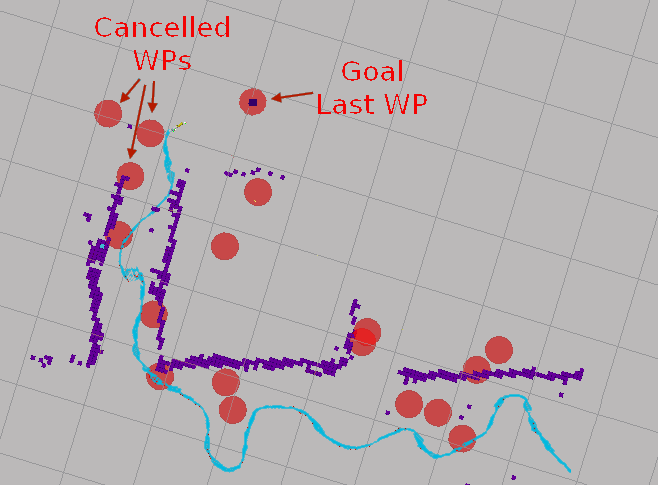
\includegraphics[width=.45\linewidth]{RealWorldOldFramework-2}} \quad
    \subfloat[Reuse last best solution]
    {\label{fig:RealWorldNewFramework}
    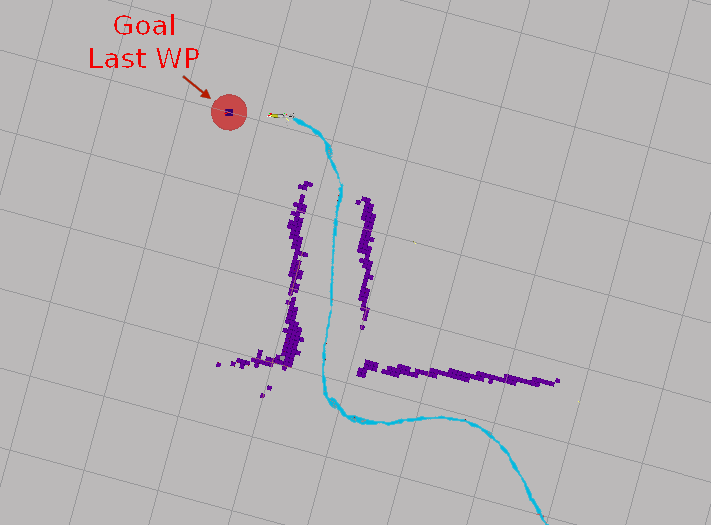
\includegraphics[width=.45\linewidth]{RealWorldNewFramework-2}}
\caption[Real-world trial to compare the \textit{anytime} computation approaches
when solving start-to-goal queries without an initial map. The test scenario
was the breakwater structure.]
{Real-world trial to compare the \textit{anytime} computation approaches
when solving start-to-goal queries without an initial map. The test scenario
was the breakwater structure where the Sparus~II had to navigate amongst two
concrete blocks to move from one side to the other of the breakwater structure.}
\label{fig:BlocksRealWorldTests}
\end{figure}

% ---------------------------------------------------------------------------
%: ----------------------- end of thesis sub-document ------------------------
% ---------------------------------------------------------------------------

